\documentclass{article}

% Evaluations & Datasets track, anonymous submission.
% For camera-ready, switch to: \usepackage[eandd, final]{neurips_2026}
% For arXiv preprint:            \usepackage[eandd, preprint]{neurips_2026}
\usepackage[eandd]{neurips_2026}

\usepackage[utf8]{inputenc}
\usepackage[T1]{fontenc}
\usepackage{hyperref}
\usepackage{url}
\usepackage{booktabs}
\usepackage{array}
\usepackage{enumitem}
\usepackage{amsfonts}
\usepackage{amsmath,amssymb}
\usepackage{nicefrac}
\usepackage{microtype}
\usepackage{xcolor}
\usepackage{graphicx}
\graphicspath{{figures/}}
% Note: algorithm + algpseudocode packages commented out during
% 2026-04-21 reorg --- sandbox texlive install lacks texlive-science.
% Currently unused (no algorithmic/algorithm environments in main.tex or
% checklist.tex). Re-enable when adding pseudocode blocks, and install
% texlive-science (apt) on the build machine.
% \usepackage{algorithm}
% \usepackage{algpseudocode}
\usepackage{subcaption}
\usepackage{multirow}
\usepackage{listings}
\usepackage{pifont}

% --- Draft helpers (remove for camera-ready) ---
\newcommand{\todo}[1]{\textcolor{red}{\textbf{[TODO: #1]}}}
\newcommand{\placeholder}[2]{%
  \begin{center}
    \fcolorbox{black}{gray!15}{%
      \parbox{#1\linewidth}{\centering\vspace{1.2cm}\textit{#2}\vspace{1.2cm}}%
    }
  \end{center}
}
% v5.6 placeholder for experimental numbers: use \expnum{X.X} for values TBD pending Experiment A
\newcommand{\expnum}[1]{\textcolor{red}{\textbf{[#1]}}}

\lstset{
  basicstyle=\ttfamily\footnotesize,
  breaklines=true,
  frame=single,
  columns=fullflexible,
  showstringspaces=false,
  language=Python,
  keywordstyle=\color{blue!70!black},
  commentstyle=\color{gray},
  stringstyle=\color{green!50!black},
}

\title{Rollout Cards for Agent Research}
% NOTE (v5.7, 2026-04-21): retitled from "Ergon: An Async Multi-Agent Gym for
% Decomposed Long-Horizon Work" to foreground the rollout-card publication-format
% contribution and anchor in the Datasheets/Model Cards genre, per the pivot
% reflected in the current abstract / §1 / §2 framing. Ergon reference
% implementation now introduced in §3 body, not in the title.

\author{%
  Anonymous Authors
}

\begin{document}

\maketitle

% ============================================================================
% v5.6 DRAFT --- fresh draft per planning/rewrite-plan.md v5.6.
% This file is the active draft (renamed from main_v55.tex during the
% 2026-04-21 repo reorg); archive/main_old.tex is the v5.4-era pre-pivot
% reference. Body sections drafted chapter-by-chapter per Execution Order
% Sessions 2-10. Appendices carried from archive/main_old.tex per Appendix
% Handling table; see TODO comments on each appendix for disposition.
% ============================================================================

% ============================================================================
% ABSTRACT
% ============================================================================
\begin{abstract}
Agent research publishes reported numbers --- accuracy, cost,
wall-clock time, gradient update --- without publishing the
rollouts those numbers were computed from. Two problems
follow. First, numbers are produced by a \emph{reporting
convention} applied to each rollout (a grading script, a
failure-handling rule, a loss function), and different
conventions applied to the same rollouts yield different
numbers. Because rollouts are discarded, these divergences
cannot be reconciled after the fact. Second, each research
community publishes only the aggregates its own conventions
compute, so replicating or extending a result along a dimension
the original harness ignored requires generating new rollouts
entirely.

We audit 50 popular training and evaluation repositories and
consolidate 37 documented cross-harness variance pairs across
task-success, cost, and timing metrics; none of the audited
harnesses surface failed rollouts alongside reported metrics.
The same pattern appears in gradient-signal computation
during training.

We propose \emph{rollout cards}: an event-sourced publication
format in which the rollout is the artefact and any reporting
convention can be applied post-hoc. Two experiments evaluate
the proposal. The first assesses whether rollout cards let
one community recover another community's key metrics from
rollouts the original harness would have discarded. The
second reconciles the 15.6pp published SWE-agent/Agentless
gap on SWE-bench Verified, attributing approximately
\expnum{C TBD}pp to a single failure-classification
convention (\texttt{no\_generation} accounting) rather than
method differences.
\end{abstract}

% ============================================================================
\section{Introduction}
\label{sec:intro}
% ----------------------------------------------------------------------------
% Session 2: Draft per Section Spec rows ``Sec.~1 opening'' + ``Sec.~1 contributions''.
% Beat: zoo-of-frameworks opening, HF-vs-Meta as single damage illustration
% (14.9pp gap between official and independent Llama 3.1 reproductions).
% Brief pointer to training-side / tracing depth without naming Sec.~2's specific
% 37-pair/50-repo numbers. Closes with three contributions bullets:
%   (1) consolidated audit of transform disagreement (Sec.~2)
%   (2) rollout-card proposal + Ergon reference implementation (Sec.~3)
%   (3) two cross-community reanalysis case studies + cross-harness reconciliation (Sec.~4)
% Target: 1.0 page total.
% ----------------------------------------------------------------------------

Language-model capabilities have grown faster than the research
ecosystem evaluating them. The infrastructure that trains and
tests these models has fragmented into a zoo of benchmark
harnesses, RL trainers, agent frameworks, and observability
middleware, each with its own conventions for how a rollout
is recorded, how a headline result is computed, and what is silently
dropped along the way. A single evaluation now routes a model's
behaviour through a stack of four or five ecosystem choices
before producing the number that appears in a paper's headline
table.

These choices are not cosmetic. Identical LLaMA-65B weights
score 63.7 on MMLU under the Berkeley evaluation code and 48.8
under \texttt{lm-evaluation-harness}: a 14.9-point gap
attributable to prompt-template and answer-extraction
conventions alone \citep{beeching2023openllm, biderman2024}.
Neither pipeline stores the raw token traces a third party
would need to recompute the score under their own convention.

The pattern extends beyond task-success metrics: cost figures
diverge by factors of two between tracing frameworks monitoring
the same API calls \citep{opentelemetry3163, langfuse12306},
wall-clock measurements differ by more than 3$\times$ between
RL trainers running the same workload \citep{hu2025openrlhf},
and training-side research has recently documented
gradient-signal differences between RL libraries applying
different loss-aggregation conventions to identical rollouts
\citep{liu2025drgrpo}. Where the underlying rollouts have been preserved, they
agree. The disagreement enters when each pipeline folds
those rollouts into a number; whichever convention the harness
happened to ship adjudicates it silently.

We argue that the field has conflated two layers:
\emph{recording} (what the rollout captures) and
\emph{reporting} (aggregates computed from it). Current practice
publishes the aggregate and discards the rollout, which makes
every convention disagreement between harnesses a disagreement
without a tiebreaker. We propose that the rollout itself be
the published artefact.

\paragraph{Contributions.} We make three contributions.

\begin{itemize}\itemsep 2pt
  \item We perform a systematic audit of 50 popular training
    and evaluation repositories at file-and-line granularity
    (\S\ref{sec:problem}). We pin every claim to a specific
    commit SHA for two-click GitHub verification.
    \textbf{We find that none of the 50 surface failed rollouts
    alongside their reported metrics. Eleven silently drop
    failures from their headline numbers, including FastChat
    (the reference scoring code behind MT-Bench and Chatbot
    Arena).} We consolidate 37 cases where the same workload
    yields different published numbers, spanning up to 14.9pp
    on task success (LLaMA-65B MMLU, Berkeley vs
    lm-evaluation-harness), 2$\times$ on cost (Anthropic cached
    tokens), and 3.13$\times$ on latency (GSM8K-GRPO epoch,
    TRL vs OpenRLHF).
  \item \textbf{We propose \emph{rollout cards}}
    (\S\ref{sec:system}): a publication-format genre in the
    Datasheets \citep{gebru2021datasheets} and Model Cards
    \citep{mitchell2019modelcards} lineage, and implement them
    as Ergon, a reference gym whose event-sourced format
    $\tau_E$ projects into the canonical trajectory formats of
    five research communities. Each projection ships an
    explicit manifest of what it drops.
  \item We evaluate the proposal with two experiments
    (\S\ref{sec:validation}). First, we show that we can record
    rollouts under one community's native convention and
    re-analyse them under another community's (MiniF2F
    binary-grading rollouts re-analysed as MCTS tree-search
    quantities; Research Rubrics scalar-score rollouts as MAS
    per-agent role differentiation). \textbf{Second, we ingest
    the published SWE-agent and Agentless submissions to
    SWE-bench Verified, re-grade both under a uniform
    convention, and find that their 15.6pp published gap
    decomposes into \expnum{C TBD}pp of harness convention
    (the treatment of no-generation outcomes) and
    \expnum{M TBD}pp of residual method difference.}
\end{itemize}

The remainder of the paper develops these contributions in
order: Section~\ref{sec:problem} the audit,
Section~\ref{sec:system} the format and its reference
implementation, Section~\ref{sec:validation} the two
experiments.

% ============================================================================
\section{Recording vs Reporting in the Current Ecosystem}
\label{sec:problem}
% ----------------------------------------------------------------------------
% Sessions 3-4: Draft per Section Spec rows ``Sec.~2.0 opening'' + ``Sec.~2.1'' + ``Sec.~2.2''.
% Structure:
%   Sec.~2.0 opening (0.25 page) --- roadmap paragraph with first-use glosses for
%     "transform"/"operator" and "recording vs reporting" per Terminology Glossary
%   Sec.~2.1 Transform disagreement across the ecosystem (1.25 pages) --- gap-first:
%     headline divergences (three-number hook: LLaMA-65B MMLU 14.9pp,
%     Anthropic cached-token 2$\times$, TRL vs OpenRLHF 3.13$\times$) with vendor-
%     acknowledgement framing, omnibus table (5-7 flagship rows across three
%     metric families, full 37-pair in Appendix B), 50-repo audit as mechanism
%     with three score-3 callouts + Inspect AI positive control, training-side
%     close with Dr. GRPO + verl #2165 (honesty discipline: these are transform
%     differences on identical rollouts, not rollout-format disparities).
%   Sec.~2.2 Different communities record different things (0.5 page, ~250 words)
%     --- prose illustration with 5 communities, dual-purpose framing
%     (illustrative + specifically what Ergon ships projections for),
%     closing bridge sentence (~40 words) naming 5 concrete needs.
%
% Drafting source: SURVEY\_master.md for Sec.~2.1 numbers, community\_recording\_needs.md for Sec.~2.2 prose.
% Target: 2.0 pages total.
% ----------------------------------------------------------------------------

Two observations recur across the agent research ecosystem.
First, the field disagrees on reported numbers computed from
what are, or could be, identical rollouts: pass rates on the
same model weights, cost totals on the same API calls, and
wall-clock times on the same training runs all differ,
sometimes substantially, depending on which \emph{reporting
convention} (grading script, aggregation rule, failure-handling
rule, timing rule, loss function) a harness applies to the
rollout. Second,
different research communities want to ask different questions
of their rollouts, and the canonical trajectory formats each
community publishes reflect which question the community is
asking. Taking the two together, \emph{recording} (what the
rollout captures) and \emph{reporting} (aggregates computed
from it) are distinct layers that should be published
separately.

\subsection{Convention disagreement across the ecosystem}
\label{sec:problem:variance}

We consolidate 37 cross-harness variance pairs where the same
workload yields different published numbers. The pairs span
three metric families (task success, cost/tokens,
latency/timing) and hold at every layer of the infrastructure
stack; in several cases the disagreement is already documented
by the infrastructure projects themselves.

On task success, HuggingFace's Open LLM Leaderboard post-mortem
documents a 14.9-point gap on LLaMA-65B MMLU between the
Berkeley evaluation code (63.7) and \texttt{lm-evaluation-harness}
(48.8): identical model weights, identical benchmark split,
different prompt-template and answer-extraction conventions
\citep{beeching2023openllm}.
On cost/tokens, OpenTelemetry PR \#3163 formalises a convention
disagreement between the OpenAI/Vertex token-accounting model
(cached tokens counted inside \texttt{input\_tokens}) and
Anthropic's (cached tokens separated into
\texttt{cache\_read\_input\_tokens} +
\texttt{cache\_creation\_input\_tokens}); the same API request
under the two conventions produces published token counts
differing by a factor of 2.0$\times$, with the delta affecting
downstream cost estimators that read \texttt{input\_tokens} as
canonical \citep{opentelemetry3163}. On latency/timing, a
head-to-head between two RL training frameworks reports
5{,}189s/epoch (TRL) versus 1{,}657s/epoch (OpenRLHF) on
GSM8K-GRPO with identical hardware, identical model, and
identical algorithm; \citet[Table 4]{hu2025openrlhf} attribute
the 3.13$\times$ gap to framework-level dispatch conventions
rather than algorithmic difference.

Several of these findings are not new. HuggingFace's
post-mortem names the MMLU variance explicitly
\citep{beeching2023openllm}. NVIDIA NeMo's documentation states
that simple-evals GPQA and \texttt{lm-evaluation-harness} GPQA
are ``distinct, non-comparable metrics'' \citep{nvidiaNemoGPQA}.
OpenTelemetry PR~\#3163 exists because the cache-token
disagreement was reaching production tracing infrastructure
\citep{opentelemetry3163}. These acknowledgements live
scattered across post-mortems, vendor documentation, and
infrastructure-project pull requests; the field has not
consolidated them or recognised them as instances of the same
phenomenon. Table~\ref{tab:omnibus} samples six flagship pairs
across the three families; the full 37-pair catalogue is in
Appendix~\ref{app:variance-catalogue}.

\begin{table}[h]
\centering
\small
\setlength{\tabcolsep}{5pt}
\caption{Flagship cross-harness variance pairs across three
metric families. Six of 37; the full catalogue with per-pair
sources is in Appendix~\ref{app:variance-catalogue}. $\Delta$
is the gap between published numbers on an identical workload;
the SWE-bench Verified Docker/Modal gap is described by the
harness authors as ``systematic'' rather than a single-number
delta \citep{swebenchHarness}.}
\label{tab:omnibus}
\begin{tabular}{@{}lllll@{}}
\toprule
\textbf{Family} & \textbf{Setup} & \textbf{Harness A} & \textbf{Harness B} & \textbf{$\Delta$} \\
\midrule
Task success  & LLaMA-65B MMLU 5-shot     & Berkeley (63.7)           & lm-eval-harness (48.8)       & \textbf{14.9pp} \\
Task success  & Mistral/Mixtral MMLU      & best prompt template      & worst prompt template        & up to \textbf{24.6pp} \\
Cost/tokens   & Anthropic cached API call & OTel input-inclusive      & Anthropic separated          & \textbf{2.0$\times$} \\
Cost/tokens   & Sonnet 3.5 on Aider       & Edit benchmark (\$0)      & Refactor+Polyglot (\$14.41)  & \textbf{\$14.41} \\
Latency/timing & SWE-bench Verified       & Docker backend            & Modal backend                & ``systematic'' \\
Latency/timing & GSM8K-GRPO, identical HW & TRL (5{,}189s/epoch)      & OpenRLHF (1{,}657s/epoch)    & \textbf{3.13$\times$} \\
\bottomrule
\end{tabular}
\end{table}

Each pair above is the default behaviour of a widely-used
harness applied to widely-used models on widely-used
benchmarks, produced without misconfiguration. Where rollouts
have been preserved, they agree. The disagreement enters at
the heuristic each harness applies at reporting time, and the
code paths producing it default to silent behaviour. We audited
50 popular training and evaluation repositories at
file-and-line granularity, pinning each to a specific SHA during
the April 2026 audit window and scoring its behaviour against five failure
scenarios (rollout exception during generation;
reward-function exception or \texttt{None}; zero-length or
unparseable output; mid-rollout environment failure; process
killed mid-rollout). Of the 50 repositories, \textbf{none
default to surfacing failures alongside metrics}: 11 exhibit
catastrophic silent dropping, 31 drop silently, and 9 log
failures but exclude them from the denominator with no
per-category counter. Four score-3 cases illustrate the pattern. FastChat, the
reference implementation behind two of the most-cited public
LLM evaluation numbers (MT-Bench and Chatbot Arena), sets
\texttt{rating = -1} on judge parse-failure and then filters
\texttt{df[df["score"] != -1]} before computing the per-model
mean and Elo, so a model that reliably produces unparseable
outputs appears to have no score rather than a bad
one.\footnote{\texttt{fastchat/llm\_judge/common.py:L175-L187};
\texttt{show\_result.py:L20, :L49};
\texttt{elo\_analysis.py:L49-L92} at SHA \texttt{587d5cf}.}

Three further cases in the same mould.
\texttt{openai/evals} retries API errors indefinitely
(\texttt{backoff.on\_predicate} with no
\texttt{max\_tries}), so any task that does not time out
eventually reports
success.\footnote{\texttt{evals/utils/api\_utils.py:10-22} at
SHA \texttt{8eac7a7}.} PrimeIntellect's \texttt{verifiers}
coerces reward-function exceptions to \texttt{0.0} and
includes them in the group-mean advantage, poisoning the
gradient for every other rollout in the
group.\footnote{\texttt{rubric.py:144-158, :208, :217, :325-333}
at SHA \texttt{e27633b}.} \texttt{ToolBench} promotes a
fraction of \texttt{give\_up\_node} trajectories to
\texttt{valid\_data=True} at random, and SFT for
\texttt{ToolLLaMA} trains on the promoted
failures.\footnote{\texttt{DFS.py:84-91};
\texttt{preprocess\_toolllama\_data.py:44-45} at SHA
\texttt{d56fdd8}.}

The best-engineered harness in the survey,
Inspect AI, defaults to \texttt{fail\_on\_error=True} and
emits per-sample error counters. Under
\texttt{fail\_on\_error=False} (common for long runs) its
denominator becomes non-errored samples with no per-category
counter.\footnote{Inspect AI at SHA \texttt{36231d6}.} Even
the positive control falls into silent bias under real-world
usage pressure.

The pattern extends to training-side computation as well, on
identical rollouts: \citet{liu2025drgrpo} documents +7.3 to
+15.7pp swings on AIME~2024 from a single loss-aggregation
convention, and verl issue~\#2165 \citep{verl2165} documents a
tokenization-channel divergence on Qwen3-4B GRPO reproduced
independently by six users. Neither is a rollout-format
disparity; both would be auditable if the rollouts were
published. We defer the full citation context to
Sec.~\ref{sec:related}.

\subsection{Different communities record different things}
\label{sec:problem:communities}

Convention disagreement does not happen in a vacuum. Five
research communities, five different canonical trajectory
formats, each shaped by the questions that community's central
analyses need to ask. \emph{Long-horizon LLM-agentic
RL} records multi-turn interactions as flat token-concatenated
rollouts with per-turn reward attribution, because the
community's central analyses are defined over exactly that
structure: LOOP's learned behaviours (consulting documentation,
minimising confabulation, recovering from setbacks)
\citep{chen2025loop} and RAGEN's Echo Trap and reward-variance
cliffs \citep{wang2025ragen}. \emph{Fixed-role multi-agent
systems} record per-agent streams with stable identities,
because MAST's 14-failure-mode taxonomy over 1{,}642 annotated
traces \citep{cemri2025mast} is computed against per-agent
attribution and full conversation histories, and its most
prevalent category (``specification and system design,''
41.8\% of failures) turns on per-agent role identification.
\emph{Hierarchical and macro-action RL} records step-indexed
trajectories with explicit option-termination events, because
deliberation cost, option domination, and premature
termination \citep{bacon2017optioncritic} are functions over
those events.

\emph{Recursive language models} record the agent-call tree
with per-node message histories and typed delegation
primitives, because ReDel's overcommitment/undercommitment
diagnostics \citep{zhu2024redel} are functions over the tree's
shape. \emph{MCTS-based LLM training} records the search tree
with per-node visit counts, Q-values, and abandoned branches,
because rStar-Math's process preference model
\citep{rstarmath2025} trains on preference pairs constructed
from exactly those abandoned branches. These five communities
are illustrative, not exhaustive: interactive theorem proving,
agentic RAG, robot learning, and embodied agents ask their own
questions of their rollouts. We focus on these five because
Ergon specifies projections for them, with the implemented
subset used in \S\ref{sec:validation} and the remaining
projections documented as extension points in
Appendix~\ref{app:integrations}. We expect the same pattern to
hold for communities whose projections we have not yet specified.

A shared substrate must therefore preserve what these examples
point to: per-agent identity, containment and termination
structure, tool-call content with reasoning channels,
experimental and environmental context, and first-class
failure recording. It must do so while supporting the
analyses different communities want to run post-hoc.

% ============================================================================
\section{Ergon: Recording as a Shared Substrate}
\label{sec:system}

\begin{figure*}[t]
\centering
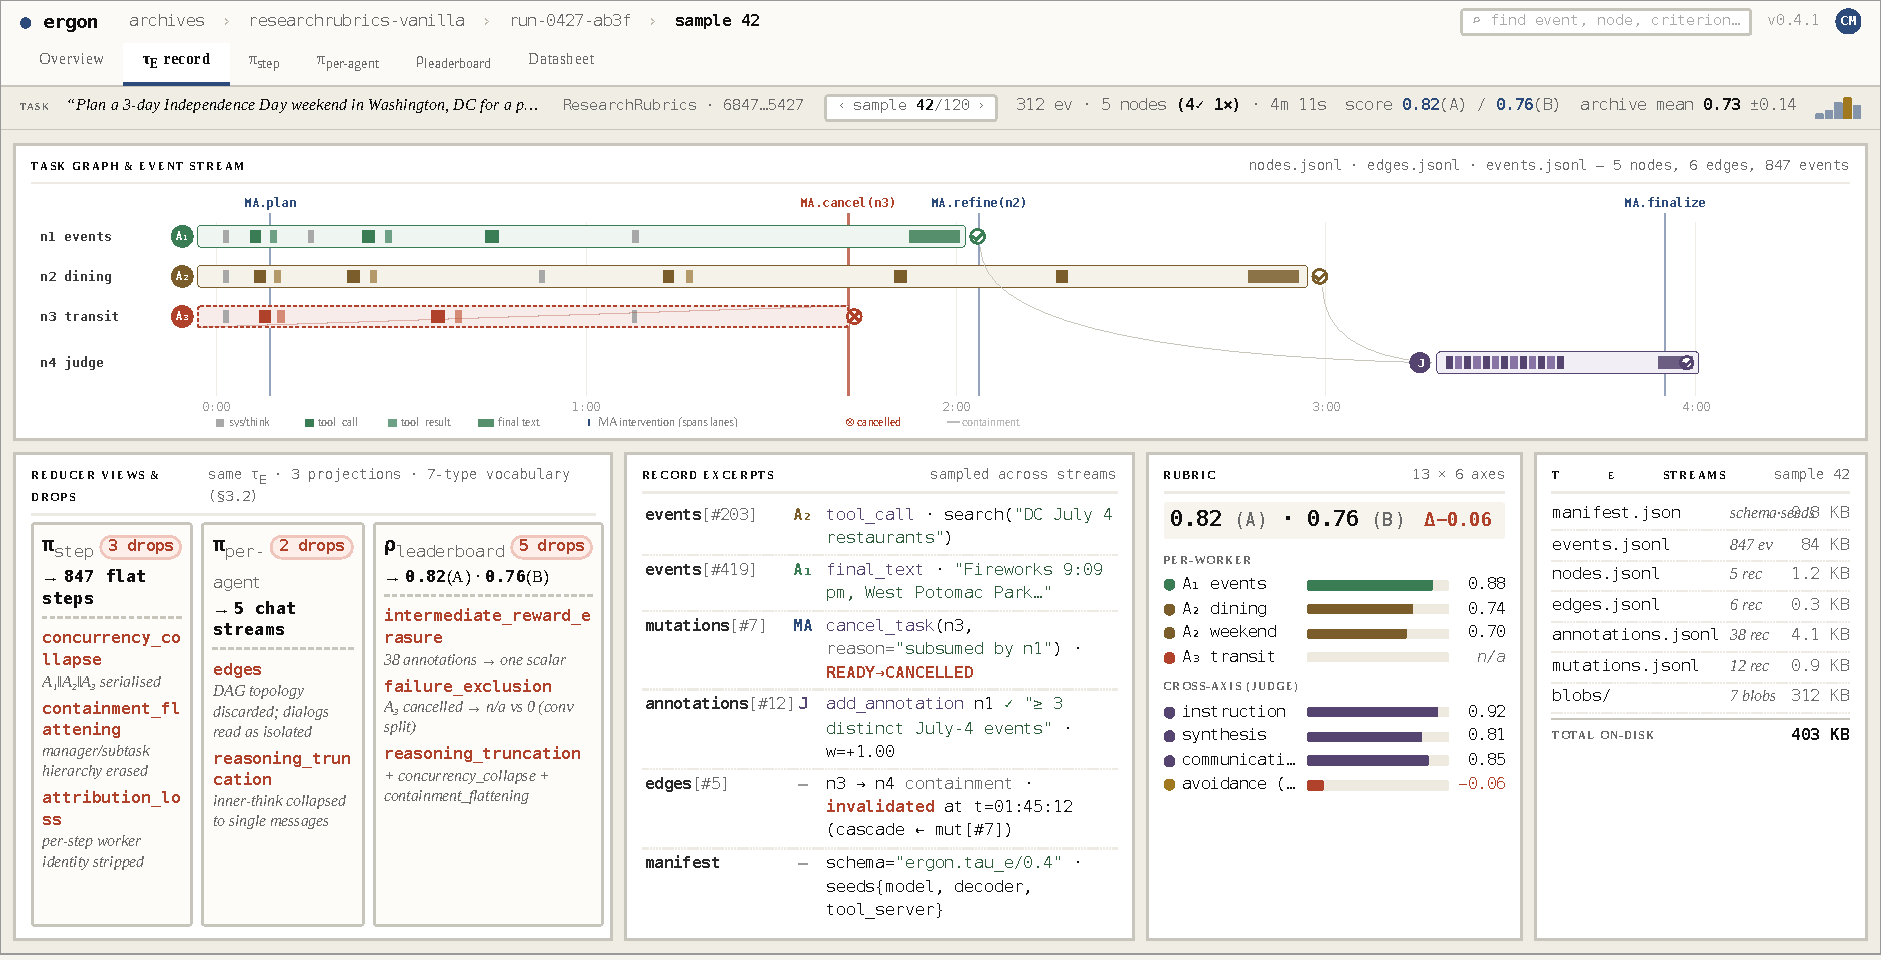
\includegraphics[width=\textwidth]{figures/ergon_dashboard.pdf}
\caption{One sample from a rollout card, viewed through the
Ergon dashboard. A $\tau_E$ record is a bundle of seven
JSONL/JSON artefacts on disk. \emph{Top:} the sample's
task-execution DAG with per-worker swim lanes and
manager-agent interventions as annotations. \emph{Bottom:}
three reducer views ($\pi_{\text{step}}$,
$\pi_{\text{per-agent}}$, $\rho_{\text{leaderboard}}$) with
their drops manifests (\S\ref{sec:system:drops}), stream
excerpts, the rubric decomposition producing the reported
scalar, and on-disk stream sizes. The dashboard is one
consumer of the format; any $\tau_E$-conformant archive loads
(\S\ref{app:system:format-spec}).}
\label{fig:dashboard}
\end{figure*}

% ----------------------------------------------------------------------------
% Sessions 5-6: Draft per Section Spec rows ``Sec.~3 opening'' + ``Sec.~3.1'' + ``Sec.~3.2'' + ``Sec.~3.3''.
% Structure:
%   Sec.~3 opening (~45 min, folded into Sec.~3.1) --- Ergon as reference implementation
%     of rollout cards, pick up Sec.~2.2's named needs through design exposition
%   Sec.~3.1 $\tau_E$ definition (0.75 page) --- event-sourced trajectory structure, each
%     field introduced with motivation mapped to Sec.~2.2's named needs and
%     community citations from community\_recording\_needs.md
%   Sec.~3.2 Projections and drops manifests (0.75 page) --- projections as transforms
%     applied post-hoc, drops manifest as methodology contribution,
%     trainer-adapters-as-transforms as training-time generalisation
%   Sec.~3.3 NEW --- Rollout cards as community standard (0.5 page) --- genre
%     positioning: Datasheets / Model Cards / Evaluation Cards precedent,
%     rollout cards as category, Ergon as reference implementation,
%     downward-compatibility claim, opt-in adoption path.
%
% Drafting source: community\_recording\_needs.md for Sec.~3.1 field motivations.
% Appendix C carries the schema detail pushed out of Sec.~3.1 body.
% Target: 2.0 pages total.
% ----------------------------------------------------------------------------

% v5.6.1 NOTE (Session 11 TODO): The Ergon-internal exposition that
% previously lived here as §3 opening, §3.1 "The Ergon trajectory", and
% §3.2 "Projection operators and drops manifests" has been moved to:
%   - Appendix C §C.1 "The τ_E trajectory representation" (the tuple
%     τ_E = (N, E, C, A, M), the five-component design exposition
%     mapping to §2.2 needs, the nine-value mutation vocabulary,
%     apply_mutation() mechanism, synchronous-transactional durability,
%     concurrency-recorded-faithfully property, bounded-loss-under-crash
%     property)
%   - Appendix C opening paragraph (projection formalism π: τ_E → (T_π, D_π),
%     typed-vocabulary erasure types, π-preserved formalism,
%     "Trainer adapters are projections" paragraph with TRL/VERL/OpenRLHF)
% Session 11 appendix work drafts these in full per the v5.6.1 plan.
%
% The body now proceeds directly from §3 section header into §3.1
% "What a rollout card contains" (format spec), §3.2 "Reporting what
% was dropped" (drops-manifest methodology), §3.3 "Ergon: a reference
% implementation" (short declarative summary), §3.4 "Rollout cards as
% a community standard" (genre positioning).

Section~\ref{sec:system} develops the proposal in three parts.
Section~\ref{sec:system:format} specifies what a rollout card
contains: the streams, the vocabulary, and the extensibility
rules. Section~\ref{sec:system:drops} introduces \emph{drops
manifests}, the methodology for reporting what each reduction
of a rollout to an aggregate discarded.
Section~\ref{sec:system:ergon} positions rollout cards in the
Datasheets and Model Cards lineage and summarises Ergon as a
reference implementation. Full system details (schema,
mutation log, trainer adapters, crash durability) are in
Appendix~\ref{app:system}.

\subsection{What a rollout card contains}
\label{sec:system:format}

A \emph{rollout card} is the portable, publication-ready
serialisation of one completed run: a self-describing archive
of JSONL streams plus a manifest and an optional blob
directory, readable by a downstream consumer without access to
the producing runtime. This is the \emph{record} side of
\S\ref{sec:problem}'s recording-vs-reporting decoupling;
\S\ref{sec:system:drops} describes the \emph{reporting} side.
Figure~\ref{fig:dashboard} shows one sample from a rollout
archive, viewed through the Ergon dashboard
(\S\ref{sec:system:ergon}); its panels preview the format's
components before we name them. The bundle is
medium-independent --- distributable as a directory, a zip, or
a HuggingFace dataset, and implementable over any storage
backend that preserves the row semantics of
Appendix~\ref{app:system:format-spec}.

Each stream addresses one of the five recording needs of
\S\ref{sec:problem:communities}. The event stream records
the reasoning-and-action trace on a monotonic per-task-execution
sequence axis as a typed vocabulary of events (full payload
union in Appendix~\ref{app:system:postgres}).
The node stream is the containment tree of task-execution
nodes, each carrying a parent pointer, a worker identity stable
across the node's lifetime, and a status drawn from an ontology
declared per-run in the annotation namespace.
The edge stream holds the dependency DAG separately from the
parent-child tree, so fire-and-forget delegation and
sibling-diamond dependencies are both representable.
The annotation stream is a namespace-keyed versioned store
that reserves one namespace for task payloads and leaves all
others to experiment code, projections, or external
instrumentation.
The mutation stream records structural change on the same
sequence axis as events, drawn from a closed nine-value
vocabulary (Appendix~\ref{app:system:mutations}); failures
appear here as status transitions rather than exceptions
routed around the recording path, the mechanism underneath
\S\ref{sec:problem:variance}'s 0-of-50 failure-surfacing
finding.
A run manifest carries metadata, a format version, and content
hashes; a blob store holds content-addressed overflow for
payloads above an inline size cap (default 64\,KB). The five streams cover the
community needs of \S\ref{sec:problem:communities} directly:
per-agent identity and failure attribution
\citep{cemri2025mast, wang2024naht}, structured reasoning-%
action traces \citep{wang2025ragen, chen2025loop}, containment
and termination semantics \citep{bacon2017optioncritic,
zhu2024redel}, and concurrent dispatch.

The format is lossless: every row in the streams corresponds
directly to a row persisted during the run, and downstream
analyses read whichever streams and namespaces they recognise.
Extensibility is via namespaces --- a team studying cross-agent
tool negotiation can claim a \texttt{tool-negotiation}
namespace and record per-edge metadata that other consumers
simply ignore, and the card remains a valid card. Ergon ships
a reference exporter (\texttt{ergon export-rollout-card
<run\_id>}), a Pydantic validator
(\texttt{ergon validate-rollout-card <path>}), and publishes
one example card per demonstration of \S\ref{sec:validation}
as a HuggingFace dataset with the camera-ready codebase.

\subsection{Reporting what was dropped}
\label{sec:system:drops}

Publishing the rollout is half of the reconciliation story;
the other half is publishing what was discarded in going from
rollout to reported number. A \emph{drops manifest} is the
typed-vocabulary record accompanying any reduction of a
rollout to an aggregate: a list of entries naming the erasure
type, the rollout element it points at, and the reported
quantity the removal affects. We draw erasure types from a
small vocabulary covering the erasures Sec.~\ref{sec:problem}
documented in practice: failure exclusion, cache-accounting
convention, intermediate-reward erasure, concurrency collapse,
containment flattening, reasoning truncation, and attribution
loss.
Figure~\ref{fig:dashboard}'s reducer-views panel displays the
drops manifests for three projections over the sample shown:
$\pi_{\text{step}}$ records three erasure classes (concurrency
collapse, containment flattening, intermediate-reward erasure),
$\pi_{\text{per-agent}}$ records two, and
$\rho_{\text{leaderboard}}$ records five.
This addresses
Sec.~\ref{sec:problem:variance}'s diagnoses directly: 0 of 50
audited repositories surface failures alongside metrics
because they do not record that failures were excluded; the 37
cross-harness variance pairs disagree untraceably because
neither harness records which erasures its own convention
applied. Making reductions legible requires naming the
erasures. Drops manifests are additive to any reducer: a team
re-grading SWE-bench trajectories under their own convention
can ship a drops manifest without adopting Ergon, and a
reviewer auditing two harnesses' disagreement on the same
rollout can compare their drops manifests directly. Ergon's
projection operators (Appendix~\ref{app:projections}) are one
instantiation, shipping a drops manifest per target format; the
vocabulary itself is the proposal.

\subsection{Ergon: a reference implementation}
\label{sec:system:ergon}

We implement the format as Ergon, an async gym with a
persistent recording substrate. Ergon hosts existing agent
frameworks (LangGraph, CrewAI, AutoGen, Claude Code) via
lightweight adapters and feeds RL trainers (TRL, VERL,
OpenRLHF) through format projections that preserve the full
trajectory underneath. Ergon writes streams synchronously
under Postgres transactions; the
\texttt{ergon export-rollout-card <run\_id>} command emits a
rollout card from any completed run, and the
Figure~\ref{fig:dashboard} dashboard is a reference reader
over any $\tau_E$-conformant archive. Ergon is one
implementation of the format: any framework matching the
specification (Appendix~\ref{app:system:format-spec}) can
publish rollout cards. Adoption is additive: a paper can ship
cards without changing its headline table, and later work can
re-analyse them under whatever convention is useful. The
paper still reports the scalar; it also publishes the rollout;
the convention that produced the scalar is separable,
inspectable, and replaceable.

% ============================================================================
\section{Experiments}
\label{sec:validation}

% ----------------------------------------------------------------------------
% Session 7 draft. Three subsections:
%   4.1 Research Questions --- RQ1 (cross-community reanalysis) + RQ2
%       (cross-harness reconciliation). Frames what §4 tests.
%   4.2 Experimental setup --- three setups: MiniF2F + Research Rubrics
%       recorded natively; SWE-bench ingested from published submissions.
%       Behavioural quantities compressed to a table.
%   4.3 Results and discussion --- RQ1 findings from MiniF2F + RR rollouts;
%       RQ2 headline finding (convention accounts for ~4pp of 15.6pp gap);
%       decomposition under Convention A and B.
%
% Placeholder numbers in \expnum{} pending:
%   - Experiment A rollouts (MiniF2F + RR, flexible-decomposition agent)
%   - Weekend 1 SWE-bench reconciliation pipeline
%
% §4.6 durability under faults --- REMOVED FROM BODY in v5.6.1. Moved to
% Appendix as Session 11 work. Body cites appendix briefly in §4.2.
% ----------------------------------------------------------------------------

\subsection{Research questions}
\label{sec:validation:questions}

We evaluate the proposal with two experiments, each addressing
one of the two problems diagnosed in \S\ref{sec:problem}:
RQ1 targets the cross-community recording mismatch of
\S\ref{sec:problem:communities}, RQ2 targets the
convention-disagreement reconciliation of
\S\ref{sec:problem:variance}. Both use rollout cards as a
shared artefact against which we apply conventions post-hoc;
neither requires re-running agents. The experimental scope is a proof of concept. Two pairings in
RQ1 and one reconciliation in RQ2 are enough to establish that
the format is structurally richer than any single community's
canonical format. We do not claim that this two-pairing scope
exhausts the community pairs for which the format is
adequate.

\paragraph{RQ1: Cross-community reanalysis.} Can a rollout
card recorded under one research community's native scorer be
consumed by a different community's scorer to recover a
quantity the original publication did not report? Positive
evidence would show that the format is rich enough to serve
communities whose questions differ from the recording
community's, directly from the rollout rather than by
re-generating trajectories under a new harness.

\paragraph{RQ2: Cross-harness reconciliation.} Can
published trajectories from two harnesses reporting different
scores on the same benchmark be ingested into a common rollout
card format, re-graded under a uniform convention, and the
reported score gap decomposed into harness-attributable and
method-attributable components? Positive evidence would show
that rollout cards provide a substrate for making otherwise
untraceable reported-number disagreements auditable.

\subsection{Setup}
\label{sec:validation:setup}

The experiments use three task families. For the first two
(MiniF2F and Research Rubrics) we run a flexible-decomposition
agent natively in Ergon to produce rollouts; these exercise
RQ1. For the third (SWE-bench Verified) we ingest rollouts from
two published submissions (SWE-agent and Agentless, both on
GPT-4o); this exercises RQ2. The two experiments draw on six
behavioural quantities, each a canonical analysis of one of the
five communities of Sec.~\ref{sec:problem:communities};
Appendix~\ref{app:quantities} catalogues the full set and we
compute three in \S\ref{sec:validation:results}. Ergon commits
every mutation synchronously
(Appendix~\ref{app:system:mutations}), so a mid-rollout crash
leaves the run graph in a well-defined partial state.

\paragraph{Cross-community reanalysis (MiniF2F, Research
Rubrics).} A single \emph{flexible-decomposition agent} runs
on both task families with a shared backbone
(\expnum{model\_target TBD}) and a turn cap of
\expnum{N TBD}. Its system prompt describes four
subtask-decomposition tools (spawn, cancel, wait-on, and
report-result) mechanically, with no task-specific strategic
guidance, so observed decomposition structure comes from the
agent rather than the prompt. Ergon records trajectories
directly as rollout cards (Sec.~\ref{sec:system:format}).

\textbf{MiniF2F} ($\sim$30 problems, Lean~4 theorem proving
\citep{zheng2022minif2f}) uses \texttt{lean\_repl} /
\texttt{lean\_check} and binary grading.
\textbf{Research Rubrics} ($\sim$30 questions, long-horizon
open-ended research) uses \texttt{web\_search} /
\texttt{read\_document} with rubric-weighted GPT-4o-mini
evaluation.

For RQ1 we pair each task family with a community whose
native scorer was \emph{not} the one the task's designers had
in mind. MiniF2F, which we record for binary proof-success,
pairs with the MCTS-based training community
\citep{rstarmath2025, feng2024restmcts}, whose quantities
include abandonment ratio by tree depth and sub-goal
semantics at abandoned nodes. Research Rubrics, which we
record for scalar rubric scores, pairs with the fixed-role
MAS community \citep{cemri2025mast}, whose quantities include
per-agent role specialisation; we capture it via
sibling-embedding distance across workers the agent spawns
from the same parent. In each pair, the target quantity is
one the source scorer discards but the recorded rollout
carries.

\paragraph{Cross-harness reconciliation (SWE-bench
Verified).} The paper's motivating gap is SWE-agent's 23.2\%
vs.\ Agentless's 38.8\% on GPT-4o-2024-05-13 (15.6pp). Both
submissions publish complete trajectories through
\texttt{swe-bench-submissions}; we ingest each into a rollout
card and re-grade under a uniform convention. The ingestion
is the main engineering step: SWE-agent ships per-instance
JSON with a flat conversation history and a denormalised
\texttt{trajectory} array, Agentless ships per-instance
Python-logger plaintext with
\texttt{ChatCompletion(\ldots)}~reprs across a seven-stage
pipeline. Each ingestion produces a drops manifest
(Appendix~\ref{app:reconciliation}) naming what the source
format could not carry, exercising the methodology of
Sec.~\ref{sec:system:drops}.

One convention choice matters enough to foreground: the
treatment of \texttt{no\_generation} outcomes, where the
harness records no agent submission. SWE-agent produces 50
such outcomes (10\% of Verified); Agentless produces 4
(0.8\%). We report under two conventions.
\emph{Convention A} excludes no-generation cases from the
denominator (isolating attempts from non-attempts);
\emph{Convention B} includes them as zeros (what the
published headlines implicitly use). The choice surfaces a
harness-level decision that neither published paper's
headline makes visible.

\subsection{Results}
\label{sec:validation:results}

Results come in three parts: RQ1a recovers MCTS-community
quantities from MiniF2F rollouts, RQ1b recovers MAS-community
quantities from Research Rubrics rollouts, and RQ2 decomposes
the SWE-agent/Agentless gap on SWE-bench Verified.

\paragraph{RQ1a: MiniF2F $\to$ MCTS-community quantities.}
We record \expnum{N TBD} MiniF2F rollouts under binary grading
and recover abandonment ratios as a function of containment
depth: at depth~1 decompositions,
\expnum{A\_1 TBD}\% are abandoned before completion; at
depth~2, \expnum{A\_2 TBD}\%; at depth~3, \expnum{A\_3 TBD}\%.
Clustering the assistant-text content at abandoned
nodes yields \expnum{K TBD} distinct sub-goal categories
(e.g.\ \expnum{category descriptions TBD}), matching the
negative-preference training signal rStar-Math's PPM uses
\citep{rstarmath2025}. We cannot derive either quantity from
the binary pass/fail the MiniF2F headline reports; we compute
both post-hoc from the rollout card's node and event streams
without re-running any proofs.

\paragraph{RQ1b: Research Rubrics $\to$ MAS-community
quantities.} We record \expnum{N TBD} Research Rubrics
rollouts under rubric-score grading and compute per-agent
sibling embedding distance: \expnum{D TBD}\% of sibling pairs
have cosine distance above \expnum{threshold TBD}, indicating
role differentiation in the sense of MAST's duplicate-agent
failure mode \citep{cemri2025mast}. The rubric-scored headline
reports a scalar per question; we can compute the
role-specialisation analysis from the same rollouts, and
\expnum{Q TBD} of \expnum{N TBD} exhibit the duplicate-agent
pattern invisible in the rubric number. Neither
task family was designed for the community whose quantities
we recover, so we claim only that the relevant quantities are
\emph{computable} from the rollouts (which current practice
of publishing community-native aggregates denies), not
numerical parity with a native harness.

\paragraph{RQ2: Cross-harness reconciliation on SWE-bench.}
Approximately \expnum{convention TBD}pp of the 15.6pp
published SWE-agent/Agentless gap on SWE-bench Verified
resolves to a single harness convention --- the treatment of
\texttt{no\_generation} outcomes, where SWE-agent produces 50
such instances (10\% of Verified) and Agentless produces 4;
the remaining \expnum{M TBD}pp is method-attributable. Neither
publication's reported number makes this classification choice
visible. Table~\ref{tab:reconciliation} decomposes the gap:
under Convention~B (the published convention, treating
no-generation as zero) the re-graded gap is
\expnum{gap\_B TBD}pp; under Convention~A (excluding
no-generation from the denominator) the remaining
gap is \expnum{gap\_A TBD}pp, attributable to how each harness
elicits patches. We take the decomposition itself to be the
primary deliverable: a gap that published as a pure method
difference turns out to have a substantial harness-convention
component, invisible without the rollout-card substrate.

\begin{table}[h]
\centering
\small
\caption{Decomposition of the 15.6pp published gap between
SWE-agent and Agentless (GPT-4o-2024-05-13, SWE-bench
Verified). Under Convention~B, no-generation outcomes count
as zeros (the published default); under
Convention~A, they are excluded from the denominator.
Ingestion drops manifests are in
Appendix~\ref{app:reconciliation}.}
\label{tab:reconciliation}
\begin{tabular}{@{}lcc@{}}
\toprule
 & \textbf{SWE-agent} & \textbf{Agentless} \\
\midrule
Published score & 23.2\% (116/500) & 38.8\% (194/500) \\
Re-graded, Convention~B & \expnum{X TBD}\% & \expnum{Y TBD}\% \\
Re-graded, Convention~A & \expnum{X' TBD}\% & \expnum{Y' TBD}\% \\
\midrule
Published gap & \multicolumn{2}{c}{15.6pp} \\
Convention-attributable (B $\to$ A delta) & \multicolumn{2}{c}{\expnum{C TBD}pp} \\
Method-attributable (under A) & \multicolumn{2}{c}{\expnum{M TBD}pp} \\
\bottomrule
\end{tabular}
\end{table}

A second observation cuts the other way. Agentless at SHA
\texttt{5ce5888} defaults missing regression-test results to
\texttt{[0]*10000} rather than surfacing them as failures
(Appendix~\ref{app:survey}, Patterns~P1 and~P4), so instances
where its own pipeline errors out are charged against the
method. The silent-drop bias therefore runs in the wrong
direction to absorb the convention gap: if anything, it
\emph{amplifies} the 15.6pp. The audit pins
\texttt{agentless/test/run\_regression\_tests.py} at the
named SHA, and a reader can verify the \texttt{[0]*10000}
default in two clicks. That SWE-agent JSON and Agentless
plaintext-log formats both ingest into the same target with
documented drops manifests (Appendix~\ref{app:reconciliation})
shows the rollout-card format accommodates heterogeneous
sources, not only data recorded natively.

% ============================================================================
\section{Related Work}
\label{sec:related}
% ----------------------------------------------------------------------------
% Session 9: Draft per Section Spec row ``Sec.~5 Related Work''. Target 0.5 page.
% Content: Datasheets / Model Cards / Evaluation Cards as direct genre
% precedent (anchored in Sec.~3.3). Transform-variance literature: Biderman et al.
% 2024 (prompt-template 24.6pp), Dr. GRPO, verl #2165 (tokenization-channel
% divergence). DAPO as secondary instance citation. Existing Sec.~5 content
% (Gym/Gymnasium, PettingZoo/JaxMARL, agent frameworks, recursive toolkits,
% schema-alignment efforts AgentOhana/VerlTool/Agent Lightning) carries
% through compressed.
% ----------------------------------------------------------------------------

We position rollout cards against four adjacent threads: the
documentation-standards genre they extend, convention-variance
documentation in evaluation and training, the
environment-and-framework landscape Ergon slots into, and
schema-alignment efforts at training-input time.

\paragraph{Genre precedent.} Rollout cards sit alongside
Datasheets for Datasets \citep{gebru2021datasheets} and Model
Cards for Model Reporting \citep{mitchell2019modelcards}:
structured artefacts published alongside a research object to
make downstream use legible. Sec.~\ref{sec:system:format}
adapts the pattern to agent trajectories.

\paragraph{Convention variance in adjacent spaces.}
\citet{biderman2024} find 24.6pp variance on LLaMA-7B MMLU
across three popular harnesses driven by prompt-template
choice. On the training side, \citet{liu2025drgrpo} document
+7.3 to +15.7pp on AIME~2024 from a single GRPO
loss-aggregation convention, and verl
issue~\#2165~\citep{verl2165} documents tokenization-channel
divergence on Qwen3-4B GRPO with six independent
reproductions. Those works identify and fix specific
conventions; the present work proposes infrastructure for
making future disagreements of this kind auditable before
they calcify.

\paragraph{Environment and framework landscape.}
Gym~\citep{brockman2016gym} and
Gymnasium~\citep{towers2024gymnasium} are the canonical
precedent for a shared evaluation interface in RL; Ergon makes
the same move at a higher level of abstraction, standardising
recording, rollout execution, and trainer integration for
decomposed long-horizon work.
PettingZoo~\citep{terry2021pettingzoo} and
JaxMARL~\citep{rutherford2024jaxmarl} extend Gym to
fixed-population multi-agent with joint actions; dynamic
population, asynchronous dispatch, mid-rollout cancellation,
and non-tree dependency sit outside that paradigm. Agent
frameworks (LangGraph~\citep{langgraph2024},
CrewAI~\citep{crewai2024}, AutoGen~\citep{wu2024autogen},
Claude Code~\citep{claudecode2024}) and inference-time
recursive toolkits (ReDel~\citep{zhu2024redel},
RLM~\citep{zhang2025rlm},
AgentOrchestra~\citep{agentorchestra2025}) run under Ergon's
substrate with automatic recording.

\paragraph{Schema alignment efforts.} Recent
surveys~\citep{yehudai2025agenteval, cemri2025mast,
yang2025agentprotocols} flag fragmentation across agent
trajectory formats, and unification efforts address it at
training time:
AgentOhana~\citep{zhang2024agentohana} standardises
trajectories into a unified training loader,
VerlTool~\citep{jiang2025verltool} aligns tool-integration
logic across agentic RL codebases, and Agent
Lightning~\citep{luo2025agentlightning} decouples LLM
generation from agent logic. Those proposals unify
\emph{training inputs}; we propose a \emph{publication
format}, with drops manifests
(Sec.~\ref{sec:system:drops}) supplying a per-format account
of what each canonical shape cannot represent.

% ============================================================================
\section{Discussion}
\label{sec:discussion}
% ----------------------------------------------------------------------------
% Session 9: Draft per Section Spec row ``Sec.~6 Discussion''. Target 0.75 page.
% Content beats:
%   (1) Policy paragraph --- publishing rollouts orders of magnitude cheaper
%       than hosting models, CERN/genomics/astronomy precedents, opt-in
%       per-researcher adoption
%   (2) Honest-limitation paragraph --- rollout cards enable DETECTION not
%       forced RESOLUTION; analogy to Datasheets/Model Cards (documentation
%       standards don't force methodological convergence)
%   (3) Dual-role community framing --- five Sec.~2.2 communities illustrate
%       general claim AND are specifically the five we ship projections for;
%       pattern generalises to ITP / agentic RAG / robot learning /
%       embodied agents but concrete support requires further projections
%   (4) Further limitations --- coverage representative, training-side
%       citation-based not reproduced, case studies single-analyst
%   (5) Future work --- transform-provenance tooling; shared transform
%       libraries; reconciliation services; projections for additional
%       communities.
% ----------------------------------------------------------------------------

We discuss four aspects of the proposal in turn: publication
cost and the adoption path, the distinction between detection
and resolution, scope limitations of the present work, and
future directions.

\paragraph{Publication cost and adoption.} Publishing rollout
cards is orders of magnitude cheaper than hosting models: a
rollout card for a completed agent run is at most a few
megabytes of text and event records, where a model checkpoint
is tens to hundreds of gigabytes. The precedent for domain-wide
rollout publishing exists elsewhere: CERN Open
Data~\citep{cernopendata} releases detector-event records from
LHC experiments; genomic consortia (1000 Genomes, UK Biobank)
publish per-individual read-level data alongside aggregate
findings; astronomy surveys (SDSS, Gaia) publish
observation-level exposures with derived catalogues. In each
case the shared artefact is the observation, not only the
analysis. Agent research can make the same move. Adoption is
opt-in per researcher and requires no coordinated ecosystem
pivot: a paper that ships a rollout card alongside its headline
number loses nothing and gains auditability; a reader who wants
to reanalyse can do so against the rollout without asking for
the original harness.

\paragraph{Detection over resolution.} Rollout cards let a
reader \emph{detect} convention disagreement. They do not by
themselves force a \emph{resolution}. A second researcher
applying a different convention to the same rollouts will
generally produce a different number than the original paper,
and we consider this a feature: the disagreement becomes
legible, because both conventions' drops manifests are
publishable and comparable, and reconcilable, because a
uniform convention can be applied to both. The Datasheets and
Model Cards analogy holds here too: documentation standards
make practice legible; they do not force methodological
convergence. We expect a field that adopts rollout cards to
have more transparent disagreements than it has today.

\paragraph{Limitations.} Coverage is representative: we draw
five communities from a long tail, audit 50 repositories from
a much larger population, and select 37 variance pairs from
the subset where documentation made comparison possible. We
cite the training-side convention-variance evidence
(Dr.~GRPO, verl~\#2165) rather than reproduce it here. The
cross-community reanalysis is single-analyst: we pair each
task family with a single target community rather than a
multi-community panel. The cross-harness reconciliation
demonstrates the format on two published submissions on one
benchmark; we leave generalisation across benchmarks and model
variants to future work.
We claim the general pattern (conventions applied without
rollouts make disagreement untraceable) is robust across
these scope bounds, but not that every specific number
generalises.

\paragraph{Future work.} Two directions. First,
convention-provenance tooling: a rollout card plus its drops
manifest is a consumable artefact for automated variance
analysis; a tool that ingests both and flags convention
divergences would make the SWE-bench finding of
Sec.~\ref{sec:validation:results} routine rather than ad hoc.
Second, training-side rollout cards:
Sec.~\ref{sec:problem:variance}'s training-side evidence
implies an analogue at the gradient-computation layer where
the loss and advantage rules play the role of the reporting
convention; we have not worked out what that looks like.

% ============================================================================
\section{Conclusion}
\label{sec:conclusion}
% ============================================================================

Agent research publishes reported numbers without the rollouts
those numbers were computed from, and the resulting coupling
between recording and reporting produces both cross-community
fragmentation and cross-harness variance that cannot be
reconciled after the fact. We proposed \emph{rollout cards}:
an event-sourced publication format in which the rollout
itself is the research artefact, and a later researcher can
apply any reporting convention (grading script, aggregation
rule, training loss) post-hoc. We introduced drops manifests as a
paper-level methodological concept accompanying any reduction
of a rollout to an aggregate, and presented Ergon as a
reference implementation at the intersection of the agent and
RL stacks. Two experiments demonstrated the proposal:
cross-community reanalysis on MiniF2F and Research Rubrics
rollouts showed that recorded trajectories carry quantities
the recording community's scorer discarded, and
cross-harness reconciliation on SWE-bench Verified showed that
a substantial fraction of a widely-published score gap
resolves to a harness convention invisible in the reported
numbers. If the field adopts the format, reported-number disagreements
become legible and auditable. That is the tractable
precondition we argue for: an ecosystem in which the field can
compare cross-community and cross-harness results on their
merits rather than on the conventions of their producers.

% ============================================================================
% BIBLIOGRAPHY
% ============================================================================
\bibliographystyle{plainnat}
\bibliography{references}

% ============================================================================
% APPENDICES
% ============================================================================
\appendix


% ----------------------------------------------------------------------------
% Appendix A --- 50-repo Failure-Handling Survey.
% Source of record: ergon_survey/SURVEY_v4.md (commit-pinned edition, April 2026).
% Structure: selection, methodology, rubric, distribution, per-repo entries
% (one-liner each; top-11 score-3 with 2-3-sentence writeup), verification
% process, coverage snapshot.
% ----------------------------------------------------------------------------

\section{50-repo Failure-Handling Survey}
\label{app:survey}

This appendix reports the code-level evidence underlying the
failure-surfacing claim in Sec.~\ref{sec:problem}. The final
sample contains 50 in-scope repositories selected by
category-stratified purposive sampling across the code paths by
which LLM-agent and LLM-training papers publish benchmark
numbers, training metrics, or leaderboard ranks. Each repository
was shallow-cloned at a pinned commit SHA during the April 2026
audit window and scored against a seven-pattern failure-handling
rubric. Every source-level claim below is backed by a
commit-pinned GitHub permalink in the supplementary survey
document \texttt{SURVEY\_v4.md}; pinned SHAs are listed in
\S\ref{app:survey:shas}.

\subsection{Repository selection}
\label{app:survey:selection}

\paragraph{Sampling frame and operational scope filter.}
The survey uses \emph{category-stratified purposive sampling}
over the code pipeline through which an LLM-agent paper
publishes a benchmark number. A repository is in-scope if and
only if, at its pinned SHA, it contains code that (a)~is
actively maintained (last commit within the past 12 months),
(b)~produces a benchmark number, training-pipeline metric, or
leaderboard rank that a published paper would cite, and
(c)~implements the result aggregation itself rather than
delegating all aggregation to a separately-versioned downstream
harness. Star-count was not used as a threshold; verified
in-scope repositories range from $\sim\!150$ stars (SciCode
164, MLAgentBench 320) to $\sim\!40$k+ (FastChat, aider),
demonstrating that the in-scope/canonical-harness filter
dominates any star-based floor. Operational scope is enforced
by two exclusions, documented as examples rather than
concealed: Online-Mind2Web was on the candidate list but
excluded after repeated clone errors prevented SHA pinning;
OpenHands was spot-checked (SHA \texttt{3b17f27}) and
documented OUT-OF-SCOPE because its evaluation harness lives in
a separately-versioned repository
(\texttt{github.com/OpenHands/benchmarks}) and the main repo
contains no result-aggregation, scoring, or denominator-handling
code. This is the operational scope filter working as intended:
OpenHands is the foundation layer (analogous to how PyTorch is
the foundation for training frameworks) and is correctly
excluded by criterion~(c).

\paragraph{Sample composition.}
The 50 repositories are grouped into five strata chosen to cover
the major places where agent-research numbers are produced:
\emph{(i)} SWE-bench-family harnesses and agent scaffolds;
\emph{(ii)} RL and agentic-RL training frameworks;
\emph{(iii)} general evaluation harnesses, LLM-as-judge systems,
and leaderboard infrastructure; \emph{(iv)} web, GUI, mobile,
scientific-agent, and ML-engineering benchmarks; and
\emph{(v)} function-calling, multi-agent, and general
agent-scaffold repositories. Selection was driven by operational
role rather than popularity: a repository was included when it
contained aggregation, scoring, denominator handling, failure
handling, reward computation, or training-metric code that could
affect a number cited in a paper.

\paragraph{Repository strata.}
\emph{(i)} SWE-bench-family harnesses and agent scaffolds
(SWE-bench, SWE-agent, mini-swe-agent, live-swe-agent,
SWE-bench\_Pro-os, SWE-smith, Agentless, aider);
\emph{(ii)}~RL training frameworks (TRL, verl, OpenRLHF, rllm,
slime, ART, Agent-R1, RAGEN, MARTI, MATPO, RL-Factory,
Trinity-RFT, ms-swift, verifiers, open-r1); \emph{(iii)}~general
eval harnesses and LLM-as-judge leaderboards (openai/evals,
simple-evals, SciCode, lm-evaluation-harness, lighteval,
inspect\_ai, FastChat/MT-Bench + Chatbot Arena, HELM, ragas,
deepeval, MTEB, promptfoo, BIG-bench); \emph{(iv)}~web/GUI,
mobile, and ML-engineering / scientific-agent benchmarks
(WebArena, VisualWebArena, OSWorld, android\_world, Mind2Web,
MLE-bench, MLAgentBench, ScienceAgentBench); and \emph{(v)}~%
function-calling and general multi-agent / scaffold repositories
(BFCL/gorilla, ToolBench, AgentBench, AgentBoard, tau-bench,
Self-rewarding-reasoning-LLM). The final sample is 50 in-scope
repositories, with two exclusions (Online-Mind2Web, OpenHands)
documented as scope-filter exemplars rather than concealed.

\subsection{Audit methodology}
\label{app:survey:method}

Each repository was shallow-cloned once into
\texttt{ergon\_survey/clones/\{repo\}} and pinned at \texttt{git
rev-parse HEAD}. The pinned SHA list in
\S\ref{app:survey:shas} is the verification baseline for every
permalink. Every citation in this appendix
resolves to
\texttt{github.com/\{owner\}/\{repo\}/blob/\{SHA\}/\{path\}\#L\{start\}-L\{end\}}
against that SHA. Each claim identifies the code path that
controls failure handling, denominator construction, reward
coercion, or result aggregation for a number the repository
can publish. Two representative per-repo reports are included
verbatim in the supplementary materials to illustrate the
template.

\subsection{Severity rubric: seven patterns of silent drop}
\label{app:survey:rubric}

Every repository was scored 0--3 against a rubric defined by
seven recurring code patterns:
\emph{(P1)} \texttt{None}-to-\texttt{0.0} reward coercion
(reward-function exception silently yields a numeric zero that
enters aggregation alongside genuine zero-reward rollouts);
\emph{(P2)} variance-based rollout filters that discard entire
rollout groups with zero std (collapse with the remaining group
in published aggregates); \emph{(P3)}
save-on-clean-exit patterns bypassed by
\texttt{KeyboardInterrupt} or early-exit cost-killers, removing
instances from the submission file rather than the denominator;
\emph{(P4)} survivor denominators --- reporting
\texttt{sum(scores) / len(scores)} over instances that reached
the aggregation step, with the pre-aggregation drop count not
preserved; \emph{(P5)} multi-turn N-destroys-1-to-N-1 patterns,
where a mid-rollout tool-call exception discards the entire
trajectory including its already-completed turns; \emph{(P6)}
LLM-judge regex-miss-to-fixed-score, where a judge returning
an unparseable response is coerced to a specific numeric score
indistinguishable from a legitimate one (e.g.\ \texttt{0.0},
\texttt{min(choice\_scores)}, \texttt{NOT\_ATTEMPTED}); and
\emph{(P7)} outcome-as-ground-truth SFT filtering, where a
downstream supervised dataset is built from only those
trajectories that scored correctly on the biased harness,
propagating the bias across a model-generation boundary. A
repository scores 3 if a single pattern is catastrophic and
observable at the headline output (the failure changes the
number a paper would cite); 2 if one or more patterns are
present but the reader cannot tell from the published CSV; 1 if
failures are logged but excluded from the denominator with no
per-category counter; 0 if all failures are surfaced alongside
metrics. No repository in the survey defaults to score 0.

\subsection{Score distribution}
\label{app:survey:distribution}

\begin{table}[h]
\centering
\small
\caption{50-repo severity scores. No repository defaults to
surfacing failures alongside metrics. OpenHands is documented
OUT-OF-SCOPE (no in-repo aggregation harness; benchmarks live
in a separately-versioned repository) and not counted in the
50. Simple-evals appears in both score-3 (SimpleQA subset) and
score-1 (non-SimpleQA subset); the $11{+}31{+}9{=}51$ listings
correspond to 50 unique repositories.}
\label{tab:survey:distribution}
\begin{tabular}{@{}clp{0.55\linewidth}@{}}
\toprule
\textbf{Score} & \textbf{Count} & \textbf{Repositories} \\
\midrule
3 & 11 & SWE-bench, openai/evals, simple-evals (SimpleQA),
VisualWebArena, ToolBench, Self-rewarding-reasoning-LLM,
PrimeIntellect verifiers, Trinity-RFT, ms-swift (GRPO), BFCL
(gorilla), FastChat (MT-Bench + Chatbot Arena) \\
\addlinespace
2 & 31 & Agent-R1, MARTI, SWE-bench\_Pro-os, RAGEN, OpenRLHF,
TRL, ART, slime, tau-bench, rllm, live-swe-agent, SWE-agent,
mini-swe-agent, MATPO, verl, AgentBoard, AgentBench,
RL-Factory, SWE-smith, lm-evaluation-harness, WebArena,
MLAgentBench, MLE-bench, lighteval, Agentless, aider, Mind2Web,
open-r1, ragas, MTEB, promptfoo \\
\addlinespace
1 & 9 & SciCode, inspect\_ai, ScienceAgentBench, android\_world,
OSWorld (harness), simple-evals (non-SimpleQA subset), HELM,
BIG-bench, deepeval \\
\addlinespace
0 & 0 & --- \\
\bottomrule
\end{tabular}
\end{table}

Inspect AI (score 1) is the positive control referenced in
Sec.~\ref{sec:problem}: its default
\texttt{fail\_on\_error=True} surfaces per-sample errors, but
the commonly-used \texttt{fail\_on\_error=False} opt-in
degrades silently with no per-category counter
(\texttt{inspect\_ai/\_eval/task/error.py:L26} and
\texttt{inspect\_ai/scorer/\_metrics/accuracy.py:L33} at SHA
\texttt{36231d6}).

\subsection{Per-repo entries}
\label{app:survey:entries}

We summarise each repository's score with a one-line evidence
pointer; the eleven score-3 repositories receive a short
2--3-sentence writeup naming the specific code site(s) and
user-visible consequence. All paths are relative to the repo
root at the pinned SHA (\S\ref{app:survey:shas}). Full
permalinks are in \texttt{SURVEY\_v4.md}.

\paragraph{Score-3 repositories (11).}

\textbf{SWE-bench.} The grading loop aggregates over
\texttt{instances\_to\_run}, filtered before aggregation
(\texttt{swebench/harness/run\_evaluation.py:L465-L470}), while
empty patches are documented as filtered
pre-submission (\texttt{docs/faq.md:L39}). A container-level
infrastructure failure stays in the denominator as a fail, but
an empty-patch instance is removed from the denominator
altogether --- and no output field separates the two cases in
the published submission.

\textbf{openai/evals.}
\texttt{backoff.on\_predicate} at
\texttt{evals/utils/api\_utils.py:L10-L22} retries transient
predicates indefinitely with no \texttt{max\_tries}, so long
runs silently absorb retry-exhaust events rather than surfacing
them. The MMMU eval treats errors as wrong answers
(\texttt{elsuite/mmmu/eval.py:L158}) and the modelgraded
classifier coerces \texttt{INVALID\_STR} to
\texttt{min(choice\_scores)}
(\texttt{elsuite/modelgraded/classify\_utils.py:L99-L101}):
three distinct P6 patterns in one library.

\textbf{simple-evals (SimpleQA subset).} The regex
fallback at \texttt{simpleqa\_eval.py:L126} defaults unparseable
responses to \texttt{NOT\_ATTEMPTED}, which the headline metric
(\texttt{accuracy\_given\_attempted = correct / (correct +
incorrect)}) then structurally excludes
(\texttt{simpleqa\_eval.py:L169-L176}). A model that hedges on
every ambiguous question looks arbitrarily accurate under this
metric --- NOT\_ATTEMPTED tasks do not appear in the
denominator.

\textbf{VisualWebArena.} An \texttt{assert "correct"
in response} at
\texttt{browser\_env/helper\_functions.py:L606} raises on
unparseable judge output, causing the outer try/except at
\texttt{run.py:L453-L461} to drop the entire task. Image-fetch
errors at \texttt{image\_utils.py:L44} propagate through the
same path. Dropped tasks are absent from the output, not
counted as failed.

\textbf{ToolBench (9/9 \textsc{verified}).} The DFS
search code at \texttt{DFS.py:L84-L91} randomly promotes a
fraction of \texttt{give\_up\_node} trajectories to
\texttt{valid\_data=True}, and SFT preprocessing at
\texttt{preprocess/preprocess\_toolllama\_data.py:L44-L45}
filters on \texttt{valid\_data} alone --- so ToolLLaMA trains
on the promoted failures. This is the paper's paradigm example
of pattern~P7 (outcome-as-ground-truth SFT).

\textbf{Self-rewarding-reasoning-LLM (4/4
\textsc{verified}).}
\texttt{infer\_math/}\allowbreak\texttt{reward\_labeling.py:L1612-L1622} grants
correctness against the ground-truth answer on the
\emph{initial} chain-of-thought; self-correction attempts must
match that \texttt{first\_reward} to be counted
(\texttt{process\_prompt\_turn3.py:L24-L62}), with a hard cap
$N=3$. There is no \texttt{try/except} anywhere in the
generation module (\texttt{gen\_hf.py}): any infra failure
silently removes a rollout.

\textbf{PrimeIntellect verifiers (5/5
\textsc{verified}).} Reward-function exceptions at
\texttt{rubric.py:L144-L158} yield \texttt{0.0}, and group
reward-function exceptions at \texttt{rubric.py:L208,~L217}
yield \texttt{[0.0]*N}. The errored zeros are then included in
the group-mean advantage at \texttt{rubric.py:L325-L333}
(\texttt{avg\_reward = sum(aggregated\_rewards) / num\_states};
\texttt{t["advantage"] = state["advantage"]}), so an
infrastructure error in one rollout biases the policy gradient
for the other rollouts in its group.

\textbf{Trinity-RFT.}
\texttt{asyncio.TimeoutError} at
\texttt{trinity/explorer/scheduler.py:L214-L216} is packaged
into \texttt{Status(ok=False,~metrics=list(),~message=\ldots)},
but the consumer path at \texttt{scheduler.py:L532-L602}
(\texttt{get\_results}) never inspects \texttt{status.ok} ---
errored payloads flow into training with \texttt{ok=False}
undetected. The over-rollout cancellation grace period
(\texttt{scheduler.py:L559-L572}, 30\,s default from
\texttt{config.py:L147}) means timeouts can also truncate
sub-tasks mid-run (\texttt{scheduler.py:L490-L506}) without
surfacing the partial-completion to the rollout log.

\textbf{ms-swift (GRPO) (8/8 \textsc{verified}).}
None-rewards are lifted to NaN at
\texttt{swift/rlhf\_trainers/grpo\_trainer.py:L359, L367,
L379}, then aggregated with \texttt{.nansum(dim=1)}
(\texttt{grpo\_trainer.py:L473}); DAPO's
\texttt{max\_resample\_times} revert (\texttt{grpo\_trainer.py:%
L684-L733}) and \texttt{overlong\_filter} mask-zeroing
(\texttt{grpo\_trainer.py:L1123-L1129}) both silently remove
rollouts from the gradient. The LLM-judge path
(\texttt{rewards/rm\_plugin.py:L216-L226}) coerces regex-parse
failures to \texttt{0.0} (pattern P6).

\textbf{BFCL / gorilla.} The weighted overall
accuracy formula in
\texttt{berkeley-function-call-leaderboard/bfcl\_eval/%
eval\_checker/eval\_runner\_helper.py:L509-L519} applies
$[10,10,10,30,40]$ weights over category runners that each
silently decrement \texttt{correct\_count} on parse failure
while leaving the denominator \texttt{len(model\_result)}
unchanged (per-category dispatch at \texttt{eval\_runner.py:%
L668}). \texttt{eval(func\_call)} exceptions become literal
\texttt{"Error during execution: \ldots"} strings
(\texttt{multi\_turn\_eval/multi\_turn\_utils.py:L97-L98}),
scored as a failed call without category attribution.

\textbf{FastChat (MT-Bench + Chatbot Arena).} FastChat is the
reference implementation for two of the most-cited public LLM
evaluation numbers: MT-Bench (LLM-as-judge single-turn and
multi-turn scoring) and Chatbot Arena (pairwise Elo ranking). A
GPT-4 or Claude judge whose response fails to match the
\texttt{[[score]]} or \texttt{[score]} regex is coerced to
\texttt{rating = -1} (P6) at
\texttt{fastchat/llm\_judge/common.py:L175-L187}; MT-Bench
aggregation then filters \texttt{df[df["score"] != -1]} before
computing the per-model mean (P2+P4) at
\texttt{show\_result.py:L20}. The pairwise path is structurally
identical: parse-failure becomes \texttt{winner = "error"}
(\texttt{common.py:L282-L304}), filtered out before Elo
computation (\texttt{show\_result.py:L49};
\texttt{elo\_analysis.py:L49-L92}). A rank swap driven by
differential parse-failure rates across judged models is not
recoverable from the headline MT-Bench or Arena Elo number ---
the attrition count is not emitted. At SHA \texttt{587d5cf}.

\paragraph{Score-2 repositories (31, one-liner each).}

\begin{description}[leftmargin=0pt,itemindent=0pt,labelindent=0pt,labelsep=0.4em,itemsep=2pt,topsep=2pt,parsep=0pt,font=\normalfont\bfseries]
\sloppy
\item[SWE-agent:] cost/kill \texttt{preds.unlink()} on
\texttt{early\_exit}/\texttt{None} removes instances from
\texttt{preds.json}
(\texttt{sweagent/run/run\_batch.py:L397-L401}).

\item[mini-swe-agent:] \texttt{finally: save()} at
\texttt{src/minisweagent/run/}\allowbreak\texttt{benchmarks/swebench.py:L171}
is bypassed by \texttt{KeyboardInterrupt} (closed issue \#329);
streaming save at \texttt{default.py:L94}.

\item[live-swe-agent:] configs never set \texttt{output\_path}
(\texttt{README.md:L71}).

\item[SWE-bench\_Pro-os:] \texttt{None} return at
\texttt{evaluation/swe\_bench\_pro\_eval.py:L346-L349} is
collapsed to \texttt{False} by callers at \texttt{:L490-L505,
L571}.

\item[AgentBench:] accuracy denominator is
\texttt{result.error is None} only
(\texttt{src/assigner.py:L368-L372}).

\item[AgentBoard:] timeouts write to \texttt{error.txt} and
never \texttt{scores.append}
(\texttt{agentboard/tasks/webbrowse.py:L275-L279}).

\item[tau-bench:] errors yield stubs with no retry
(\texttt{tau\_bench/run.py:L89-L96}).

\item[SWE-smith:] broad \texttt{except} at
\texttt{scripts/collect\_trajs.py:L77-L79};
\texttt{random.sample} cap at
\texttt{scripts/combine\_trajs.py:L86-L91}.

\item[TRL:] \texttt{None}$\to$NaN$\to$\texttt{nansum} at
\texttt{trl/trainer/grpo\_trainer.py:L1228-L1230, L2132}.

\item[verl:] PRIME reward timeouts$\to$\texttt{0.0} at
\texttt{verl/workers/reward\_manager/}\allowbreak\texttt{prime.py:L37-L42, L83};
missing \texttt{return\_exceptions=True} at
\texttt{verl/experimental/agent\_loop/}\allowbreak\texttt{agent\_loop.py:L603}
(closed issue \#5956).

\item[OpenRLHF:] remote RM
exception$\to$\texttt{reward=None}
(\texttt{openrlhf/utils/agent.py:L298-L299}; open issue
\#1139).

\item[rllm (Berkeley Sky):] no-valid-trajectory episodes
dropped at \texttt{rllm/engine/}\allowbreak\texttt{agent\_workflow\_engine.py:L266};
\texttt{dropped\_episodes} never written into
\texttt{DataProto.meta\_info} at \texttt{:L249} (open issue
\#382).

\item[slime:] oversampling discard + zero-std filter at
\texttt{slime/rollout/sglang\_rollout.py:L449}.

\item[ART:] \texttt{drop\_zero\_advantage\_trajectories=True}
default at \texttt{src/art/preprocessing/tokenize.py:L158}.

\item[Agent-R1:] length-truncated trajectories published as
complete at
\texttt{agent\_r1/agent\_flow/agent\_env\_loop.py:L120-L129}.

\item[RAGEN:] variance filter skips whole training step at
\texttt{ragen/trainer/}\allowbreak\texttt{agent\_trainer.py:L1054-L1056}.

\item[MARTI:] dynamic filter drops saturated groups at
\texttt{marti/trainer/ppo\_trainer.py:L481-L510}.

\item[MATPO:] MCP + judge failures$\to$reward 0.0 at
\texttt{verl/tools/mcp\_tool.py:L137, L150} and
\texttt{llm\_judge.py:L265, L312, L356}.

\item[RL-Factory:] malformed tool
JSON$\to$\texttt{continue} at
\texttt{verl/workers/rollout/}\allowbreak\texttt{sglang\_rollout/}\allowbreak\texttt{sglang\_rollout.py:L914-L916};
PRIME timeouts$\to$0.0 at \texttt{prime.py:L141-L146}.

\item[lm-evaluation-harness:] left-truncate with
\texttt{eval\_logger.warning} only
(\texttt{lm\_eval/models/huggingface.py:L1360-L1368}; closed
issues \#3419, \#3352, \#3161, \#1323).

\item[WebArena:] outer \texttt{except Exception:
log-and-continue} at \texttt{run.py:L217-L364}; headline
\texttt{sum(scores) / len(scores)} over survivors at
\texttt{run.py:L365}; \texttt{env.step} swallow with
\texttt{terminated=False} on infra failure at
\texttt{browser\_env/envs.py:L239-L248}.

\item[MLAgentBench:] subprocess
crash$\to$\texttt{"EnvError"} string at
\texttt{low\_level\_actions.py:L181-L220} +
\texttt{environment.py:L328-L334}; hard-coded magic baselines
at \texttt{plot.py:L249-L274}; fresh random GT per call at
\texttt{fathomnet/eval.py:L11}.

\item[MLE-bench:] aggregation \texttt{pad\_missing=False}
drops incomplete seeds at
\texttt{experiments/aggregate\_grading\_reports.py:L69-L135};
\texttt{MedalInfo} logic at
\texttt{mlebench/grade\_helpers.py:L123-L133}.

\item[lighteval:] LiteLLM returns empty
\texttt{LitellmModel}\allowbreak\texttt{Response()} on Azure
content-filter and retry-exhaust
(\texttt{litellm\_model.py:L243, L254}); empty response scored 0
at \texttt{metrics\_sample.py:L151-L152}; left-truncate prompts
without \texttt{truncated\_}\allowbreak\texttt{tokens\_count} at
\texttt{vllm\_model.py:L374-L397}.

\item[Agentless:] missing regression-test results default to
\texttt{[0]{*}10000} at
\texttt{agentless/test/run\_regression\_tests.py} (P1+P4),
collapsing absent results into a vector of 10k zeros;
\texttt{\_post\_process\_multifile\_repair} returns an empty
tuple on exception, and SWE-bench filters empty patches
pre-submission (\texttt{docs/faq.md:L39}), removing the
instance from the denominator. Directly relevant to
\S\ref{sec:validation}'s RQ2 reconciliation of the
SWE-agent/Agentless 15.6pp gap (at SHA \texttt{5ce5888}).

\item[aider:] benchmark-runner broad \texttt{except} at
\texttt{benchmark/benchmark.py:L666-L676} stores the exception
as \texttt{\{"exception": \ldots\}} row; aggregation at
\texttt{:L502-L512} divides by \texttt{len(rows)}, so
exception rows contribute 1 to the denominator and 0 to the
numerator without surfacing the infra-flake count.

\item[Mind2Web:] \texttt{IndexError} on out-of-bounds choice
index caught at
\texttt{src/action\_prediction/metric.py:L203-L209}
(\texttt{logger.info}-only), falls through to score-0 + kept in
denominator (P1); \texttt{src/action\_prediction/}%
\texttt{dataloader.py:L277} applies a train-only positive-%
candidate filter, creating a train/eval data-distribution
asymmetry (P7).

\item[open-r1:] E2B broad \texttt{except} at
\texttt{src/open\_r1/rewards/code\_providers.py:L107-L112}
coerces sandbox exceptions to \texttt{[0.0]{*}len(scripts)}
rewards with print-only surface; MorphProvider identical
pattern at \texttt{:L248-L249}; IOI/Codeforces paths enter
TRL's \texttt{None}$\to$\texttt{nansum} pipeline via
\texttt{:L396-L397, L449-L450}.

\item[ragas:] Pydantic parser fallback at
\texttt{ragas/prompt/pydantic\_prompt.py:L315-L334} (self-fix
loop raises \texttt{RagasOutputParserException}); executor
broad \texttt{except} returns \texttt{float("nan")} at
\texttt{ragas/executor.py:L64-L86}; \texttt{safe\_nanmean} at
\texttt{ragas/utils.py:L46-L55} silently shrinks the
denominator by the NaN count across faithfulness, answer-%
relevancy, and context-precision metrics.

\item[MTEB:] leaderboard aggregate filters out models with any
NaN task score at \texttt{mteb/leaderboard/\_create\_table.py:%
L136-L149} (P4 selection bias); per-language aggregates at
\texttt{mteb/results/task\_result.py:L526-L563} compute over
produced scores with no attempt-vs-score coverage counter.

\item[promptfoo (TypeScript):] any LLM-judge parse failure
coerced to \texttt{\{pass: false, score: 0\}} at
\texttt{src/matchers/llmGrading.ts:L499, L515} (P6); fail
helpers at \texttt{src/matchers/shared.ts:L25-L38} return the
same hardcoded score indistinguishably from legitimate zeros;
provider-error path at \texttt{src/evaluator.ts:L1046-L1051}
produces \texttt{score: 0} without a \texttt{providerErrored}
flag.
\end{description}

\paragraph{Score-1 repositories (9, one-liner each).}

\begin{description}[leftmargin=0pt,itemindent=0pt,labelindent=0pt,labelsep=0.4em,itemsep=2pt,topsep=2pt,parsep=0pt,font=\normalfont\bfseries]
\sloppy
\item[SciCode:] partial-submission aggregation at
\texttt{eval/scripts/}\allowbreak\texttt{test\_generated\_}\allowbreak\texttt{code.py:L125-L127}.

\item[inspect\_ai:] \texttt{fail\_on\_error=True} by default
(\texttt{\_eval/task/error.py:L26}), but
\texttt{fail\_on\_error=False} opt-in degrades silently
(\texttt{scorer/\_metrics/accuracy.py:L33}).

\item[ScienceAgentBench:] swallows
\texttt{EvaluationError/BuildImageError/Exception}
(\texttt{evaluation/harness/run\_evaluation.py:L118-L136});
discards \texttt{timed\_out} flag (\texttt{:L113}); GPT-4o
judge regex-miss$\to$score 0 at
\texttt{gpt4\_visual\_judge.py:L70-L72}.

\item[android\_world:] \texttt{np.nan} +
\texttt{DataFrame.mean} asymmetric drop at
\texttt{task\_evals/task\_eval.py:L249-L259} and
\texttt{android\_world/suite\_utils.py:L544-L558, L681-L698}.

\item[OSWorld (harness):] bare-\texttt{except} ``Time
limit exceeded'' at \texttt{run.py:L205-L218};
\texttt{env.evaluate()} \texttt{FileNotFoundError}$\to$0 at
\texttt{desktop\_env/desktop\_env.py:L485-L487};
Verified-subset non-comparability disclaimer at
\texttt{README.md:L36}.

\item[simple-evals (non-SimpleQA subset):] honest grading on
multi-choice, regex miss$\to$wrong on GPQA/MMLU (see
Appendix~\ref{app:variance-catalogue}, Smoking-Gun~\#2).

\item[HELM:] \texttt{Stat.add(None)} silently skips None
results at \texttt{src/helm/benchmark/metrics/statistic.py:L35};
judge parse returns \texttt{None} at \texttt{gpt4\_audio\_}%
\texttt{critique\_metrics.py:L70-L72} and is absorbed by the
\texttt{Stat.add(None)} skip. The per-scenario attrition rate
is recoverable from the full output JSON but is not in the
headline report (at SHA \texttt{83bde5c}).

\item[BIG-bench:] aggregate metric computation at
\texttt{bigbench/api/results.py:L560-L576} uses
\texttt{statistics.mean(d[m] for d in per\_task if m in d)},
silently shifting the denominator by the count of tasks that
did not produce metric \texttt{m}. Per-task results are
preserved in raw output so the shift is recoverable, but the
headline mean does not emit a coverage counter (at SHA
\texttt{092b196}).

\item[deepeval:] \texttt{JSONDecodeError} on LLM-judge output
re-raised as \texttt{ValueError} at
\texttt{deepeval/utils.py:L405-L413} and caught broadly by the
test-runner; \texttt{safe\_a\_measure} at
\texttt{deepeval/progress\_context.py:L299-L305} catches any
metric-evaluation exception. Per-test failure messages are
surfaced but parse-failure rates are not aggregated into a
headline counter (at SHA \texttt{f917b5a}).
\end{description}

\subsection{Verification}
\label{app:survey:verification}

Every source-level claim in this appendix is tied to a pinned
commit SHA and a line-level permalink in the supplementary
survey document. Claims were retained only when the cited lines
directly supported the stated failure-handling behaviour. The
audit therefore fixes both the repository version and the exact
code location being asserted, making each entry independently
checkable without relying on moving default branches.

\subsection{Pinned commit SHAs}
\label{app:survey:shas}

Every permalink in this appendix resolves against the
following pinned commits. Repositories are grouped by survey
stratum; full 40-character SHAs and line-level permalinks are
provided in the supplementary survey document.

\emph{SWE-bench-family harnesses and agent scaffolds.}
SWE-bench \texttt{f7bbbb2}; SWE-agent \texttt{0f4f3bb};
mini-swe-agent \texttt{bc85a45}; live-swe-agent
\texttt{8d7dd86}; SWE-bench\_Pro-os \texttt{0c64e26};
SWE-smith \texttt{9b74ac0}; Agentless \texttt{5ce5888};
aider \texttt{f09d7065}.

\emph{RL and agentic-RL training frameworks.}
TRL \texttt{88826fd}; verl \texttt{6eeb571}; OpenRLHF
\texttt{64c1cc4}; rllm \texttt{ea623cc}; slime
\texttt{5b688aa}; ART \texttt{679b236}; Agent-R1
\texttt{38bdfc1}; RAGEN \texttt{20daedc}; MARTI
\texttt{a2fe2c7}; MATPO \texttt{3c41d62}; RL-Factory
\texttt{d0abc1d}; Trinity-RFT \texttt{9051d63}; ms-swift
\texttt{c4902f3}; verifiers \texttt{e27633b}; open-r1
\texttt{1416fa0}.

\emph{General evaluation harnesses and leaderboard infrastructure.}
openai/evals \texttt{8eac7a7}; simple-evals \texttt{ee3b031};
SciCode \texttt{e3158ea}; lm-evaluation-harness
\texttt{c1c4bea}; lighteval \texttt{10b9104}; inspect\_ai
\texttt{36231d6}; FastChat \texttt{587d5cf}; HELM
\texttt{83bde5c}; ragas \texttt{298b6827}; deepeval
\texttt{f917b5a}; MTEB \texttt{9363ea75}; promptfoo
\texttt{3dc5843}; BIG-bench \texttt{092b196}.

\emph{Web, GUI, mobile, scientific-agent, and ML-engineering benchmarks.}
WebArena \texttt{dce0468}; VisualWebArena \texttt{89f5af2};
OSWorld \texttt{c7e54d2}; android\_world \texttt{d9c569f};
Mind2Web \texttt{33bd95c}; MLE-bench \texttt{2451bcb};
MLAgentBench \texttt{5d71205}; ScienceAgentBench
\texttt{1cf1375}.

\emph{Function-calling, multi-agent, and general agent-scaffold repositories.}
gorilla (BFCL) \texttt{6ea5797}; ToolBench \texttt{d56fdd8};
AgentBench \texttt{d1e4a10}; AgentBoard \texttt{bb7255e};
tau-bench \texttt{59a200c}; Self-rewarding-reasoning-LLM
\texttt{372bea9}. The out-of-scope observation (OpenHands,
documented as a scope-filter exemplar) is pinned at
\texttt{3b17f27}.

\subsection{Coverage snapshot}
\label{app:survey:coverage}

The final sample contains 50 in-scope repositories and two
documented exclusions. It spans SWE-bench-family harnesses,
agent scaffolds,
RLHF trainers, agentic-RL trainers, multi-agent RL, web/GUI
agents, mobile agents, ML-engineering benchmarks,
scientific-agent benchmarks, function-calling benchmarks,
general eval frameworks, LLM-judge infrastructure, autonomous
coding assistants, RAG-eval frameworks, embedding/retrieval
benchmarks, red-team/prompt-eval tooling, and
rejection-sampling SFT pipelines.
The severity distribution is 11 score-3 entries, 31 score-2
entries, 9 score-1 entries, and 0 score-0 entries. Because
\texttt{simple-evals} is scored separately for SimpleQA and
non-SimpleQA behaviour, these 51 entries correspond to 50
unique repositories. Seven silent-drop patterns
covering reward coercion, rollout filtering, bypassed saves,
survivor denominators, partial-trajectory drops, LLM-judge
parse$\to$fixed score, and outcome-as-ground-truth SFT
filters.
The audit contains 50 pinned SHAs and approximately 160
verified source citations. Every code claim in this appendix is a
commit-pinned two-click audit: if any claim fails to hold up
at its permalink, that is a bug in this appendix, not a vague
disagreement about code that has since moved --- the SHAs fix
the audit target.

% ----------------------------------------------------------------------------
% Appendix B NEW --- 37-pair variance catalogue. Draft fresh in Session 11.
% Source: SURVEY\_master.md. Structure: full table organised by metric family
% --- task success (22 pairs), cost/tokens (9 pairs), latency/timing (6 pairs).
% Near-misses section for leads not meeting evidence bar.
% ----------------------------------------------------------------------------

\section{37-pair Variance Catalogue}
\label{app:variance-catalogue}

This appendix enumerates the 37 cross-harness variance pairs
sampled in Table~\ref{tab:omnibus}, organised by metric family:
22 task-success pairs (\S\ref{app:vc:task}), 9 cost/token
pairs (\S\ref{app:vc:cost}), and 6 latency/timing pairs
(\S\ref{app:vc:latency}). Four task-success benchmarks are
then examined in \emph{smoking-gun} detail
(\S\ref{app:vc:smoking}) --- same dataset, multiple in-survey
implementations, different numbers on identical workloads.
Training-side evidence beyond the rollout interface
(Dr.\ GRPO, DAPO, TRL's five GRPO variants, verl~\#2165) is
consolidated in \S\ref{app:vc:training}. A de-duplication log
(\S\ref{app:vc:dedup}) records which family each pair is
counted in, and \S\ref{app:vc:nearmisses} catalogues leads that
did not meet the evidence bar.

\subsection{Evidence hierarchy}
\label{app:vc:hierarchy}

Every pair is graded against the same four-tier evidence
hierarchy, uniform across the three metric families:

\begin{enumerate}
\item \textbf{Tier 1 --- strongest.} Same model and workload;
published numbers disagree across two harnesses. (Direct
empirical evidence.)
\item \textbf{Tier 2.} Explicit vendor or framework
documentation acknowledging the convention difference between
harnesses. (Vendor-admission-equivalent.)
\item \textbf{Tier 3.} Code-level convention divergence with
no cross-framework normalization, published under the same
metric name. (Structural divergence visible at source.)
\item \textbf{Tier 4.} Maintainer issue-tracker statement that
the convention differs from another framework. (Maintainer-%
acknowledged divergence.)
\end{enumerate}
Anything weaker is demoted to near-misses
(\S\ref{app:vc:nearmisses}). Every pair below cites either a
numeric delta, a vendor acknowledgement, a code-level
convention divergence, or a maintainer statement.

\subsection{Task-success pairs (22)}
\label{app:vc:task}

Same model weights, same benchmark split, different published
accuracy depending on which harness computed the aggregate.

\begin{table}[h]
\centering
\footnotesize
\setlength{\tabcolsep}{3pt}
\caption{22 task-success variance pairs. $\Delta$ is the gap
between published numbers on an identical workload. ``post-%
mortem'' refers to the HuggingFace Open LLM Leaderboard
post-mortem \citep{beeching2023openllm}.}
\label{tab:vc:task}
\begin{tabular}{@{}l>{\raggedright\arraybackslash}p{0.12\linewidth}>{\raggedright\arraybackslash}p{0.13\linewidth}>{\raggedright\arraybackslash}p{0.14\linewidth}>{\raggedright\arraybackslash}p{0.16\linewidth}>{\raggedright\arraybackslash}p{0.12\linewidth}>{\raggedright\arraybackslash}p{0.16\linewidth}@{}}
\toprule
\textbf{\#} & \textbf{Model} & \textbf{Benchmark} &
\textbf{Harness A} & \textbf{Harness B} &
\textbf{$\Delta$} & \textbf{Source} \\
\midrule
T1  & LLaMA-65B         & MMLU 5-shot   & Berkeley orig.       & lm-eval-harness    & 14.9pp         & post-mortem \\
T2  & LLaMA-30B         & MMLU 5-shot   & Berkeley orig.       & lm-eval-harness    & 12.6pp         & post-mortem \\
T3  & Falcon-40B        & MMLU 5-shot   & Berkeley orig.       & lm-eval-harness    & 10.5pp         & post-mortem \\
T4  & Llama-3.1-70B-Inst & MMLU-Pro     & Meta self (CoT)      & OLL v2 / lighteval & $\sim$18.5pp   & Meta card vs OLL \\
T5  & Qwen2.5-72B       & MMLU-Pro      & Self-report          & OLL v2             & $\sim$22pp     & Qwen docs vs OLL \\
T6  & GPT-4o (24-05-13) & SWE-b.\ Verified & SWE-agent         & Agentless 1.5      & 15.6pp         & swe-b.\ subs.\ S3 \\
T7  & Claude 3.5 Sonnet & SWE-b.\ Verified & Anthropic Tools   & OpenHands CA 2.1   & 4.0pp          & SWE-b.\ leaderb. \\
T8--T13 & Various       & SWE-b.\ Lite/Ver. & Various          & Various            & 3.4--19.6pp   & SWE-b.\ leaderb. \\
T14 & Mistral-7B        & MMLU (prompt) & Template A           & Template B         & up to 24.6pp   & Biderman et al.\ \\
T15 & Mixtral-8x7B      & MMLU (prompt) & Template A           & Template B         & up to 24.6pp   & Biderman et al.\ \\
T16 & Mistral-7B        & ARC (prompt)  & Template A           & Template B         & up to 24.6pp   & Biderman et al.\ \\
T17 & Llama-3.1-70B     & MATH          & Meta (full test)     & Leaderboard (500)  & label collision & Meta vs leaderb. \\
T18 & Claude 3.5 Sonnet & MATH          & ``MATH''             & ``MATH''           & label overload & multi-source \\
T19 & Llama-3.1-70B     & GPQA          & simple-evals         & lm-eval-harness    & vendor admis.\ & NVIDIA NeMo \\
T20 & Llama-3.1-70B     & GPQA          & Self-report          & Leaderboard        & cross-harness  & Meta + leaderb.\ \\
T21 & Llama-3.1-70B     & Various       & Meta model card      & Meta \texttt{eval\_details.md} & micro vs macro & Meta own docs \\
T22 & Llama-3.1-70B     & Various       & \texttt{acc\_char}   & full-string match  & convention    & Meta own docs \\
\bottomrule
\end{tabular}
\end{table}

T1 (LLaMA-65B MMLU 14.9pp) is the flagship single pair ---
identical weights, different published score, explicitly
discussed in a HuggingFace post-mortem. T6 (GPT-4o SWE-bench
Verified 15.6pp) is the target of the reconciliation
experiment in Sec.~\ref{sec:validation:results}:
trajectories for both runs are in the public SWE-bench
submissions S3 bucket, making the reconciliation tractable.
T14--T16 (Biderman et al.) are not cross-harness pairs but
within-harness prompt-template pairs, included because the
24.6pp gap is the strongest published evidence that the
instrument-level variance is at least as large as the
signals it purports to measure.

\subsection{Cost / token pairs (9)}
\label{app:vc:cost}

Same model, same workload, different published token counts or
dollar costs depending on which tool applies which convention.
Table~\ref{tab:vc:cost} summarises; for numerical examples and
code-level references see the supplementary survey document and
the cost-latency divergence report in supplementary materials.

\begin{table}[h]
\centering
\footnotesize
\setlength{\tabcolsep}{3pt}
\caption{9 cost / token-accounting variance pairs. Same model,
same workload, different published numbers.}
\label{tab:vc:cost}
\begin{tabular}{@{}l>{\raggedright\arraybackslash}p{0.15\linewidth}>{\raggedright\arraybackslash}p{0.22\linewidth}>{\raggedright\arraybackslash}p{0.22\linewidth}>{\raggedright\arraybackslash}p{0.28\linewidth}@{}}
\toprule
\textbf{\#} & \textbf{Setup} & \textbf{Harness A} &
\textbf{Harness B} & \textbf{$\Delta$} \\
\midrule
C1 & Anthropic w/ \texttt{cache\_control}  & OTel \texttt{input\_tokens} (inclusive) & Anthropic-native (exclusive)       & 2.0$\times$ inflation (260{,}421 vs 130{,}213) \\
C2 & Claude + cache\_control               & LiteLLM cost estimator                  & Anthropic Console billing          & +68\% overestimate (\$0.091 vs \$0.054) \\
C3 & Claude (streaming) + cache-hit        & LangChain.js accumulator                & single \texttt{message\_delta}     & exactly 2$\times$ cache\_read          \\
C4 & SWE-b.\ V.\ retry-firing task         & SWE-agent (every attempt)               & mini-swe-agent (last attempt)      & 30--100\% per-task overstatement       \\
C5 & Anthropic/OpenAI prompt-cache         & inspect\_ai (cache-aware, tiered)       & 7 peer harnesses (no cache parse)  & up to 90\% on cached portion           \\
C6 & Aider leaderboards (same model date)  & Aider Edit                              & Aider Refactor / Polyglot          & \$0 $\to$ \$14.41 (same model)         \\
C7 & Same rollout batch, GRPO training     & verl \texttt{loss\_agg\_mode=}\allowbreak\texttt{token-mean} & verl \texttt{seq-mean-}\allowbreak\texttt{token-sum}  & different gradient magnitudes          \\
C8 & Cross-vendor ``tokens used''          & tiktoken (\texttt{o200k\_base})         & Anthropic BPE                      & $\sim$10\% systematic                  \\
C9 & OpenAI reasoning models (o1/o3)       & harness reading \texttt{completion\_}\allowbreak\texttt{tokens} only & harness reading \texttt{..details.}\allowbreak\texttt{reasoning\_tokens} & silent under-report \\
\bottomrule
\end{tabular}
\end{table}

\paragraph{Code-level sources.}
{\footnotesize\raggedright
\textbf{C1:} OpenTelemetry PR~\#3163; Langfuse issue~\#12306.
\textbf{C2:} BerriAI/litellm issue~\#9812.
\textbf{C3:} langchainjs issue~\#10249.
\textbf{C4:} \texttt{sweagent/agent/models.py} L744--L838;
\texttt{minisweagent/models/litellm\_model.py} L80--L93.
\textbf{C5:} \texttt{inspect\_ai/model/\_openai.py} L776--L782;
\texttt{inspect\_ai/model/\_model.py} L2085--L2091;
\texttt{inspect\_ai/model/\_providers/anthropic.py} L1137--L1169.
\textbf{C6:} \texttt{edit\_leaderboard.yml},
\texttt{refactor\_leaderboard.yml},
\texttt{polyglot\_leaderboard.yml} in \texttt{Aider-AI/aider}.
\textbf{C7:} \texttt{verl/trainer/ppo/core\_algos.py} L1168--L1195.
\textbf{C8:} tiktoken and Anthropic tokenizer documentation;
openai/tiktoken issue~\#474.
\textbf{C9:} OpenAI API reference for reasoning-model
\texttt{usage.completion\_tokens\_details}.
\par}

C1 is the flagship: OpenTelemetry PR~\#3163 formalises the
Anthropic/OpenAI/Vertex convention disagreement at the
observability-middleware layer, and Langfuse issue \#12306
exhibits the numerical 260{,}421-vs-130{,}213 gap on a single
request. C6 is the flagship intra-vendor disagreement: the
same organisation's three leaderboards (Edit, Refactor,
Polyglot) publish \$0, \$8.46, and \$14.41 for the same model
on comparable tasks, with no convention statement in any of
the three YAMLs.

\subsection{Latency / timing pairs (6)}
\label{app:vc:latency}

Same workload, same hardware, different published wall-clock
times depending on which harness's timer wraps which phase.

\begin{table}[h]
\centering
\footnotesize
\setlength{\tabcolsep}{3pt}
\caption{6 latency / wall-clock variance pairs. Clock-start
and clock-stop differ across harnesses that log the same
metric name.}
\label{tab:vc:latency}
\begin{tabular}{@{}l>{\raggedright\arraybackslash}p{0.17\linewidth}>{\raggedright\arraybackslash}p{0.22\linewidth}>{\raggedright\arraybackslash}p{0.22\linewidth}>{\raggedright\arraybackslash}p{0.26\linewidth}@{}}
\toprule
\textbf{\#} & \textbf{Setup} & \textbf{Harness A} &
\textbf{Harness B} & \textbf{$\Delta$} \\
\midrule
L1 & SWE-b.\ V.\ (same task)       & Docker backend                       & Modal backend                       & systematic Modal inflation            \\
L2 & OSWorld (same task)          & \texttt{lib\_run\_single.py}         & \texttt{scripts/python/}\allowbreak\texttt{run\_maestro.py} & $\ge$30\,s (hardcoded sleep) + 5--15\,s VM start \\
L3 & GRPO step timer              & TRL \texttt{training\_}\allowbreak\texttt{step} (grad+opt only) & verl \texttt{marked\_timer(}\allowbreak\texttt{"step")} (full epoch) & up to 5$\times$ on rollout-dominated runs \\
L4 & Qwen2.5-7B GSM8K-GRPO, same HW & TRL                                & OpenRLHF                            & 3.13$\times$ (5{,}189\,s vs 1{,}657\,s) \\
L5 & GRPO throughput              & verl \texttt{perf/throughput} (excl.\ padding) & TRL effective-token throughput      & different numerators on same HW        \\
L6 & inspect\_ai timers           & \texttt{sample\_working\_time}       & \texttt{sample\_waiting\_time}      & ambiguity declared in-tool            \\
\bottomrule
\end{tabular}
\end{table}

\paragraph{Code-level sources.}
{\footnotesize\raggedright
\textbf{L1:} \texttt{swebench/harness/docker\_utils.py}
L203--L217 vs
\texttt{swebench/harness/modal\_eval/run\_evaluation\_modal.py}
L307--L319.
\textbf{L2:} \texttt{lib\_run\_single.py} \#L616 vs
\texttt{scripts/python/run\_maestro.py} \#L351.
\textbf{L3:} \texttt{trl/trainer/grpo\_trainer.py} L1111--L1120;
\texttt{verl/trainer/ppo/metric\_utils.py} L313--L346.
\textbf{L4:} arXiv:2501.03262 Table~4; EMNLP-demos 2025.
\textbf{L5:} \texttt{verl/trainer/ppo/metric\_utils.py}
L337--L345.
\textbf{L6:} \texttt{inspect\_ai/\_util/working.py}.
\par}

L4 is the flagship: published, peer-reviewed, same hardware,
same model, same algorithm --- a 3.13$\times$ wall-clock gap
attributable to framework-level dispatch rather than algorithm
difference. L1 and L2 are in-repository disagreements: both
backends in SWE-bench Verified and both harnesses in OSWorld
ship under the same repo at the same commit, reporting the
same metric name, with no statement that the two are not
comparable.

\subsection{Smoking-gun benchmarks: same dataset, multiple in-survey implementations}
\label{app:vc:smoking}

Four benchmarks are implemented in 3--4 surveyed repositories
each. Below, each implementation's grading site and
failure-handling semantics are read off at the pinned SHAs
(\S\ref{app:survey:shas}). For each benchmark, a single
realistic failure mode produces a different headline number in
each implementation --- and none of the implementations emits
a counter disclosing which regime it fell into.

\paragraph{Smoking-Gun~\#1: SWE-bench (4 implementations).}
\emph{Official SWE-bench} grades via \texttt{bad\_codes} =
\{APPLY\_PATCH\_FAIL, RESET\_FAILED, TESTS\_ERROR,
TESTS\_TIMEOUT\}
(\texttt{swebench/harness/grading.py:L61-L70};
\texttt{constants/\_\_init\_\_.py:L80-L89}) with empty patches
pre-filtered from submission (\texttt{docs/faq.md:L39}). Container
timeout stays in the denominator as a fail; empty-patch
instances are removed entirely. \emph{PrimeIntellect verifiers}
reads the same \texttt{bad\_codes} set but wraps
\texttt{test\_spec} fetching in a 5$\times$ tenacity retry; any
uncaught exception flows through \texttt{rubric.py:L144-L158}
to \texttt{0.0} and enters the group-mean advantage baseline
--- a container timeout can bias the policy gradient for the
other rollouts in its group rather than merely decrementing
the numerator. \emph{SWE-agent} delegates grading to
\texttt{sb-cli submit}
(\texttt{sweagent/run/hooks/swe\_bench\_evaluate.py:L42-L55});
the pre-submission \texttt{unlink} at
\texttt{run\_batch.py:L397-L401} removes crashed or
cost-killed instances from \texttt{preds.json} entirely, so
server-side grading sees a smaller denominator instead of a
failed row. \emph{mini-swe-agent} has no local grading; its
\texttt{finally: save()} at
\texttt{benchmarks/swebench.py:L171} is bypassed by
\texttt{KeyboardInterrupt} (closed issue \#329), also
producing an absent-from-submission pattern. On one realistic
mid-test Docker timeout, the four harnesses report: Official
$0/N$, verifiers $1/N$ (possible retry recovery), SWE-agent
$0/(N-1)$, mini-swe-agent $0/(N-1)$. Inspect~AI has \emph{no
SWE-bench bridge} at the pinned SHA.

\paragraph{Smoking-Gun~\#2: GPQA (3 implementations).}
\emph{simple-evals} at \texttt{gpqa\_eval.py:L59} uses
\texttt{re.search(ANSWER\_PATTERN\_MULTICHOICE, response\_text)}
and \texttt{extracted\_answer = match.group(1) if match else
None}; a regex miss --- which a hedging response triggers ---
is scored 0 and stays in the denominator. \emph{lm-evaluation-%
harness} uses log-likelihood of the gold-choice token over the
various \texttt{gpqa\_*\_zeroshot.yaml} /
\texttt{\_n\_shot.yaml} / \texttt{\_cot\_*.yaml} tasks; the
model does not generate free text in the scored branch, so
hedging is immune, but silent left-truncation at
\texttt{huggingface.py:L1360-L1368} still affects long
contexts. \emph{lighteval} scores via the standard pipeline at
\texttt{tasks/tasks/gpqa.py} with aggregation through
\texttt{info\_loggers.py:L326-L400}; API retry-exhaust or
content-filter yields an empty
\texttt{LitellmModelResponse()} (\texttt{litellm\_model.py:%
L243, L254}), scored as wrong via
\texttt{metrics\_sample.py:L151-L152} (\texttt{if not pred:
return 0}). On a single hedging model output: simple-evals~0,
lm-eval-harness likely correct, lighteval~wrong --- three
different headline accuracies from the same model reasoning.
Inspect~AI has \emph{no GPQA task file} at the pinned SHA.

\paragraph{Smoking-Gun~\#3: MATH / MATH-500 (3
implementations).} \emph{simple-evals} at
\texttt{math\_eval.py:L55} calls \texttt{check\_equality(self.%
equality\_checker, row["Answer"], extracted\_answer)}, which
itself calls the LLM equality checker; an API failure raises
(dropping the sample) or is coerced to 0 by the outer handler.
\emph{lighteval} uses majority@n with a symbolic
\texttt{math\_normalizer} over \texttt{tasks/tasks/math\_500.py}
and \texttt{math.py}; normalizer exceptions are caught upstream
and scored wrong at
\texttt{metrics\_sample.py:L151-L152}. \emph{PrimeIntellect
verifiers} routes reward functions through
\texttt{rubric.py:L144-L158}; exceptions become \texttt{0.0}
and enter the group advantage baseline. On a LaTeX edge case
such as \texttt{\textbackslash frac\{1\}\{2\}} versus
\texttt{0.5}: simple-evals's LLM judge may call these equal,
lighteval's normalizer may not, and verifiers's reward
exception enters training as an errored zero --- same
completion, three different outcomes.

\paragraph{Smoking-Gun~\#4: MMLU (3 implementations).}
\emph{simple-evals} (\texttt{mmlu\_eval.py}) extracts answers
by regex on generated text --- same miss-is-wrong pattern as
GPQA. \emph{lm-evaluation-harness}
(\texttt{lm\_eval/tasks/mmlu}: 12+ variants spanning main,
redux, pro, flan, etc.) uses log-likelihood over A/B/C/D
tokens with \texttt{acc}/\texttt{acc\_norm}; silent prompt
truncation at \texttt{huggingface.py:L1360-L1368} logs the
truncated-prompt sample as a complete result.
\emph{lighteval} uses exact-match on the choice label
(\texttt{tasks/tasks/mmlu.py}), with left-truncation at
\texttt{vllm\_model.py:L374-L397} warning but recording no
\texttt{truncated\_tokens\_count}. On a long-context MMLU-Pro
prompt that overflows a 4k model: simple-evals generates a
regex answer against the truncated prompt the model saw
(right or wrong depending on the content);
lm-eval-harness left-truncates and logs as complete (silently
wrong); lighteval left-truncates, records no truncation
counter, and logs as complete (silently wrong, with no
recoverable audit trail). Three implementations, three
behaviours, no \texttt{n\_prompt\_truncated} counter in any
output.

\subsection{Training-side evidence beyond the rollout interface}
\label{app:vc:training}

Operator disagreement extends into the gradient-signal
computation at training time. The paper cites these as
published findings rather than original contributions.

\textbf{Dr.\ GRPO} \citep{liu2025drgrpo} corrects only the
loss-aggregation convention --- the length-normalization bias
documented in ``all popular open-source PPO implementations''
--- and reports +7.3 points on AIME 2024 vs SimpleRL-Zero-7B
and +15.7 points on AIME 2024 vs Prime-Zero-7B, with no change
to data, model, or algorithm. \textbf{DAPO}
\citep{yu2025dapo} is a catalogue of framework-level defaults
(zero-std group filter, token-vs-sequence loss aggregation,
decoupled clip ranges) that had to be flipped to match
DeepSeek-R1; the paper reports 50 points on AIME 2024 for
Qwen2.5-32B on the defaults-flipped run. All three defaults
are silently different across TRL, verl, and OpenRLHF.
\textbf{TRL's own library} ships five mutually-incompatible
GRPO variants --- \texttt{grpo}, \texttt{dr\_grpo},
\texttt{dapo}, \texttt{bnpo}, and
\texttt{importance\_sampling\_level}$\in$\{\texttt{token},
\texttt{sequence}\} --- in a single config file
(\texttt{trl/trl/trainer/grpo\_config.py:L228-L243,
L668-L677}); two papers reporting ``we trained with GRPO on
task X'' are structurally non-comparable without specifying
which variant. \textbf{verl~\#2165} \citep{verl2165} is a
tokenization-channel divergence on Qwen3-4B GRPO where the
training-side FSDP tokenizer inserts
\texttt{<think>\textbackslash n\textbackslash n</think>} into
assistant turns that the rollout engine (vLLM~/~SGLang) never
saw, shifting the assistant-turn token mask by tens of tokens
across $\sim$40k-token conversations. The finding is reproduced
by six independent users on the thread, upstream-confirmed in
QwenLM/Qwen3~\#1826 and Qwen/Qwen3-1.7B HF discussion~\#9, and
guarded separately by verl's own
\texttt{tokenization\_sanity\_check\_mode} (distinct from the
dtype guard in discussion~\#5984) --- proving that tokenization-%
class mismatch exists as a separate failure mode even when all
upstream dtypes match.

\textbf{Silent rollout-dropping mechanisms (beyond the 50-repo
audit).} verl~\#1170 (rollouts silently return empty strings,
training proceeds); OpenRLHF~\#1108 (reward curves diverge
between vLLM 0.8.1 and 0.8.3 on the same seed); verl
discussion~\#5984 (tool built specifically to detect silent
per-token log-prob divergence between training FSDP and vLLM
rollouts); ms-swift~\#9096 (gemma-4 rollouts return garbage,
training continues). \textbf{Numerical-layer evidence.} BF16
backends have been documented to produce divergent log-probs
between training and rollout engines even with identical
weights (``Defeating the Training-Inference Mismatch via
FP16,'' arXiv:2510.26788); the vLLM engineering blog documents
separate backends breaking the on-policy assumption of
policy-gradient methods; THUDM's \texttt{slime} ships a
\texttt{train\_infer\_mismatch\_helper} because divergence is
expected.

\subsection{De-duplication log}
\label{app:vc:dedup}

Several findings could plausibly appear in more than one
family. For audit transparency we record where each is counted
and why:

\begin{itemize}
\item \textbf{Dr.\ GRPO}, \textbf{DAPO}, \textbf{TRL's five
GRPO variants}: counted in \S\ref{app:vc:training}
(training-side); not in \S\ref{app:vc:cost} despite touching
per-step token accounting. Rationale: the load-bearing claim is
about gradient signal, not token counts.
\item \textbf{verl~\#2165} (Qwen3 tokenization-channel
divergence): counted in \S\ref{app:vc:training} (training-%
side); not in \S\ref{app:survey} despite involving silent
per-rollout mismatch. Rationale: Appendix~\ref{app:survey}
audits \emph{failure-handling} patterns; verl~\#2165 is a
\emph{convention-disagreement} finding, structurally closer to
Dr.\ GRPO than to \texttt{try/except/return None}.
\item \textbf{TRL vs OpenRLHF 3.13$\times$ wall-clock} (L4):
counted in \S\ref{app:vc:latency}; not in
\S\ref{app:vc:training} despite the training-pipeline context.
The headline delta is wall-clock, not gradient signal.
\item \textbf{verl \texttt{loss\_agg\_mode} variants} (C7):
counted in \S\ref{app:vc:cost}; not in \S\ref{app:vc:latency}
despite affecting per-step timing.
\item \textbf{verl throughput metric} (L5): counted in
\S\ref{app:vc:latency}; not in \S\ref{app:vc:cost} despite
involving token counting.
\item \textbf{inspect\_ai \texttt{sample\_working\_time} vs
\texttt{sample\_waiting\_time}} (L6): counted in
\S\ref{app:vc:latency}; not in \S\ref{app:survey} despite
inspect\_ai's role as the positive control for
failure-handling.
\end{itemize}
No finding is counted twice across the 37 pairs.

\subsection{Near misses}
\label{app:vc:nearmisses}

Leads that did not meet the evidence bar
(\S\ref{app:vc:hierarchy}) but warrant human follow-up.

\textbf{Cost / tokens.} Anthropic
\texttt{/v1/messages/count\_tokens} versus tiktoken estimate
--- Anthropic publishes a dedicated counting endpoint,
community harnesses routinely substitute tiktoken for speed,
the endpoint returns different numbers on the same input;
documented but no published benchmark pair with materially
different totals attributable to this choice. Anthropic
\texttt{/cost} underreport vs dashboard (anthropics/claude-%
code~\#1063): intra-vendor, not cross-harness. HuggingFace
Open LLM Leaderboard v1$\to$v2 transition (including the
lighteval vs lm-eval-harness switch): full methodology change
with no explicit ``efficiency numbers not comparable across
versions'' statement.

\textbf{Latency.} HELM \texttt{efficiency.json} publishes
per-model latency/throughput but is frozen at pre-2023 models
with no modern cross-comparison. OpenAI vs Azure OpenAI
latency differences on the same model are documented but with
no published benchmark pair.

\textbf{Task success.} Anecdotal ``our replication differs
from the original paper'' issue-tracker threads that do not
cite a specific convention difference.

% ----------------------------------------------------------------------------
% Appendix C --- Projection Operators to Community Trace Shapes.
% EDIT per Appendix Handling table: cut pseudocode from six subsections
% (terminology-glossary-enforced principle under v5.6), keep Target/Preserved/
% Dropped paragraphs. EXPAND with $\tau_E$ schema details moved out of Sec.~3.1 body
% during Session 11 appendix work.
% Content initially carried verbatim from main.tex lines 983-1388, then edited.
% ----------------------------------------------------------------------------

\section{Projection Operators to Community Trace Shapes}
\label{app:projections}

This appendix defines each projection
$\pi: \tau_E \to (T_\pi, D_\pi)$ whose structural preservation
properties appear in Table~\ref{tab:preservation}. For each we
give: (i) the target trace format as a formal object;
(ii) pseudocode for the projection function operating on
$\tau_E = (N, E, C, A, M)$; (iii) the drops manifest $D_\pi$ as
a list of typed erasure records; (iv) a characterisation of which
substrate structure the projection preserves. Reference
implementations are in the released codebase; the pseudocode here
is the specification, not the implementation. Each drops manifest
record is a tuple
$(\textit{erasure\_type}, \textit{element\_ref},
\textit{metric\_class})$ per~\S\ref{app:projections}.

Figure~\ref{fig:sixproj} gives the visual summary before the
definitions: one SWE-Bench Verified rollout $\tau_E$ rendered
through all six projections, with each projection's drops
manifest overlaid.

\begin{figure}[h]
\placeholder{0.95}{%
  \textbf{Figure C.1: One SWE-Bench Verified trajectory, six
  representations.} Centre: substrate state $\tau_E$ for one
  rollout, rendered with containment tree (vertical), dependency
  DAG (horizontal edges), reasoning-log events (timeline), and
  typed mutations (marked). Five surrounding panels: the same
  trajectory under each projection below. Drops manifest records
  overlaid on each panel, colour-coded by erasure type (concurrency
  collapse, cancellation erasure, edge deletion, containment
  flattening, reasoning truncation, attribution loss).
  $\pi_{\text{step}}$ and $\pi_{\text{per-agent}}$ each show
  large shaded regions (structural erasure);
  $\pi_{\text{call-tree}}$ serialises concurrent siblings into an
  ordering; $\pi_{\text{macro}}$ collapses sub-tree reasoning
  into aggregate effects; $\pi_{\text{json-log}}$ matches the
  substrate up to schema encoding.
}
\caption{One SWE-Bench Verified trajectory rendered through all
six representations, with drops manifests overlaid.}
\label{fig:sixproj}
\end{figure}

\paragraph{Preservation, operationally.} We use ``projection''
informally --- a function that loses information. A behavioural
quantity $\mu: \tau_E \to \mathbb{R}$ is \emph{$\pi$-preserved}
iff there exists a computable $g$ such that
$g(\pi(\tau)) = \mu(\tau)$ for all $\tau$; that is, $\mu$ factors
through $\pi$. Table~\ref{tab:preservation} records three cases
per (projection, quantity) pair: (i)~\textbf{preserved}
(\ding{51}): such a $g$ exists given $T_\pi$'s canonical schema
alone; (ii)~\textbf{erased} (\ding{55}): no such $g$ exists
because $T_\pi$ lacks the relevant channel; (iii)~\textbf{partial}
($\sim$): $g$ exists on a subset of $\tau_E$ but not universally,
admitting a numeric preservation fraction
$\rho_{\pi,\mu} \in (0,1)$ whose computation requires running
$\pi$ against a trajectory corpus and is beyond the scope of this
paper. Each cell is therefore a concrete question (``does $g$
exist given $T_\pi$'s schema?'') rather than a qualitative
judgement.

\begin{table}[h]
\centering
\footnotesize
\setlength{\tabcolsep}{4pt}
\caption{Structural preservation matrix. Rows: the six projections
defined below plus the raw substrate $\tau_E$. Columns: the six
community-native behavioural quantities of \S\ref{sec:validation}
(\textbf{Step-ret}: step-indexed return under episode mask, long-horizon
LLM-agentic RL~\citep{chen2025loop, wang2025ragen};
\textbf{Opt-term}: option termination frequency,
HRL/macro-action~\citep{bacon2017optioncritic}; \textbf{Call-dep}:
call-tree depth distribution, recursive LMs~\citep{zhu2024redel};
\textbf{Sib-dist}: per-agent sibling embedding distance, fixed-role
MAS~\citep{cemri2025mast}; \textbf{MCTS-ent}: node visit entropy
across frontier, MCTS-based training~\citep{rstarmath2025,
feng2024restmcts}; \textbf{Async-dp}: dispatch-and-wait rate,
async MAS). \ding{51}~=~preserved under $\pi$;
\ding{55}~=~$T_\pi$ has no channel that could carry the elements
contributing to the quantity; $\sim$~=~partially preserved. Cells
follow from the projection pseudocode in
\S\S\ref{app:proj:step}--\ref{app:proj:json-log}.}
\label{tab:preservation}
\begin{tabular}{@{}lcccccc@{}}
\toprule
\textbf{Projection} & \textbf{Step-ret} & \textbf{Opt-term} & \textbf{Call-dep} & \textbf{Sib-dist} & \textbf{MCTS-ent} & \textbf{Async-dp} \\
\midrule
$\pi_{\text{step}}$      (long-horizon RL)    & \ding{51} & \ding{55} & \ding{55} & \ding{55} & \ding{55} & \ding{55} \\
$\pi_{\text{macro}}$     (hierarchical)       & $\sim$    & \ding{51} & \ding{51} & \ding{55} & \ding{55} & $\sim$    \\
$\pi_{\text{call-tree}}$ (recursive LM)       & $\sim$    & $\sim$    & \ding{51} & $\sim$    & \ding{55} & \ding{55} \\
$\pi_{\text{per-agent}}$ (fixed-role MAS)     & $\sim$    & \ding{55} & \ding{55} & \ding{51} & \ding{55} & $\sim$    \\
$\pi_{\text{mcts}}$      (search-tree)        & \ding{55} & \ding{55} & $\sim$    & \ding{55} & \ding{51} & \ding{55} \\
\midrule
$\pi_{\text{json-log}}$  (production ref.)    & \ding{51} & \ding{51} & \ding{51} & \ding{51} & \ding{51} & \ding{51} \\
$\tau_E$                 (Ergon raw)          & \ding{51} & \ding{51} & \ding{51} & \ding{51} & \ding{51} & \ding{51} \\
\bottomrule
\end{tabular}
\end{table}

Table~\ref{tab:preservation} reads off the projection definitions
below. The pattern is consistent: the five community projections
each preserve their own native quantity on the diagonal and
(mostly) erase the others; $\pi_{\text{step}}$ carries no
structural channel beyond the token-indexed step sequence and so
erases every non-self-community question;
$\pi_{\text{json-log}}$ preserves every quantity by construction
but is not a training target for any of the five communities.
The off-diagonal $\sim$ cells (e.g.,
$\pi_{\text{call-tree}} \times$~Sib-dist) indicate cases where
$T_\pi$ carries some but not all of the channel $\mu$ requires:
$\pi_{\text{call-tree}}$ preserves sibling \emph{relations} but
not the reasoning-log content embeddings MAST's role-differentiation
metric computes over.

A methodological note: Table~\ref{tab:preservation} asks whether
$\mu$ factors through $\pi$, not whether any proxy for $\mu$
does. A weaker proxy claim --- say, ``fraction of episodes
terminated before the environment terminates'' as a surrogate for
option termination under $\pi_{\text{step}}$ --- may survive
erasure of the canonical quantity. Whether such a proxy counts
as the same claim is a judgement the framework does not
adjudicate; it establishes only that the canonical $\mu$, as
defined over $\tau_E$, does not factor through $\pi$.

\subsection{$\pi_{\text{step}}$: step-indexed $(o_t, a_t, r_t)$ tuples}
\label{app:proj:step}

\paragraph{Target format.} A token-indexed flat prompt-response
tensor pair, matching the \texttt{DataProto}
schema~\citep{sheng2024hybridflow} consumed by VERL, OpenRLHF,
and TRL: $(\texttt{prompts}, \texttt{responses},
\texttt{attention\_mask}, \texttt{response\_mask},
\texttt{token\_level\_scores}, \texttt{advantages})$, where
\texttt{token\_level\_scores} is a per-token reward tensor of
shape $[\text{batch}, \text{response\_length}]$. Equivalently, a
sequence $T_{\text{step}} = [(o_1, a_1, r_1), (o_2, a_2, r_2),
\ldots]$ where each step corresponds to a token position and
$r_t \in \mathbb{R}$ is its assigned reward. Multi-turn
interactions are handled by concatenating turn tokens into one
flat response per rollout; no per-turn identity is preserved in
the tensor shape.

\paragraph{Projection pseudocode.}
\begin{lstlisting}
def pi_step(tau_E):
    N, E, C, A, M = tau_E
    T_step = []
    D = []  # drops manifest
    # Walk M in sequence order; emit one step per
    # (assistant_text | tool_call -> tool_result) pair
    # from the root node's reasoning log only.
    root = find_root(N)
    events = [e for e in C if e.node_id == root.id]
    for e in events_by_sequence(events):
        if e.kind == "assistant_text" or e.kind == "tool_call":
            a_t = e.payload
            o_t = next_observation_after(e, C)
            r_t = reward_for(e, A)   # from annotation store
            T_step.append((o_t, a_t, r_t))
    # Record drops
    for n in N:
        if n.id != root.id:
            D.append(("containment_flattening", n.id, "depth"))
    for edge in E:
        D.append(("edge_deletion", edge.id, "tree_likeness"))
    for m in M:
        if m.kind in ("node.added", "node.status_changed")
            and m.node_id != root.id:
            D.append(("cancellation_erasure"
                      if "cancel" in m.payload else
                      "attribution_loss",
                      m.id, "late_cancel"))
    for e in C:
        if e.node_id != root.id:
            D.append(("reasoning_truncation", e.id, "role_diff"))
    return T_step, D
\end{lstlisting}

\paragraph{Preserved.} The root worker's linear sequence of
assistant text and tool interactions with its own environment.
\paragraph{Dropped.} Everything else: the containment tree beyond
the root, all dependency edges, all cross-worker causal structure,
all cancellation events as typed policy actions (they appear, if
at all, only as the absence of subsequent children), per-worker
identity beyond the root, and the reasoning logs of all
non-root workers.

\subsection{$\pi_{\text{per-agent}}$: per-worker streams with partner annotations}
\label{app:proj:per-agent}

\paragraph{Target format.} A mapping from worker identifier to a
per-worker stream:
$T_{\text{per-agent}} = \{ w_i \mapsto \sigma_i \}_{i=1}^{k}$,
where each $\sigma_i$ is a per-worker stream of observations and
actions for worker $w_i$ under a topology declared before the
rollout, optionally annotated with role tags or partner-type
beliefs. This shape covers fixed-role multi-agent LLM systems,
MARL with a centralised critic, proposer/critic debate setups,
and --- as a special case of coordination under partner
uncertainty --- ad hoc teamwork~\citep{mirsky2022aht,wang2024naht}.
Cross-stream references are limited to dependency edges between
streams, which the format does not natively carry.

\paragraph{Projection pseudocode.}
\begin{lstlisting}
def pi_per_agent(tau_E):
    N, E, C, A, M = tau_E
    workers = group_by(N, key=lambda n: n.assigned_worker_key)
    T_per_agent = {}
    D = []
    for w, nodes in workers.items():
        stream = []
        events = [e for n in nodes for e in C if e.node_id == n.id]
        for e in events_by_sequence(events):
            if e.kind in ("assistant_text", "tool_call",
                          "tool_result"):
                stream.append(event_to_stream_record(e))
        T_per_agent[w] = stream
    # Drops
    for n in N:
        if n.parent_node_id:
            D.append(("containment_flattening", n.id, "depth"))
    for edge in E:
        src_w = worker_of(edge.src, N)
        dst_w = worker_of(edge.dst, N)
        if src_w != dst_w:
            D.append(("edge_deletion", edge.id, "tree_likeness"))
    for m in M:
        if m.kind == "node.status_changed"
            and m.payload.status == "cancelled":
            D.append(("cancellation_erasure", m.id, "late_cancel"))
    return T_per_agent, D
\end{lstlisting}

\paragraph{Preserved.} Per-agent trajectory streams indexed by
agent identity, matching the shape MARTI~\citep{marti2025}
distributes to individual policy trainers. Partial concurrency
information: a consumer comparing wall-clock timestamps across
streams can detect overlapping activity. Partial role
differentiation: embedding analysis across the per-agent streams
remains possible, though the stream-identity boundary is now a
projection artefact rather than a containment-tree fact.

\paragraph{Dropped.} The format is agent-major rather than
work-major: task-level structure --- which subtask is shared
across which agents, which agents are blocked on each other's
dispatches, which branches were cancelled as typed events --- is
carried by the workflow class in systems like MARTI (Multi-Agent
Debate, Mixture-of-Agents, Chain-of-Agents) and is not
recoverable from the per-agent streams alone. Specifically:
containment depth (the parent-child relation flattens to stream
identity); cross-worker dependency edges; cancellation as a
typed action (worker terminations appear only as stream
endings); async dispatch-and-wait (the dispatch is in one
stream, the result in another, with no expressible causal link).

\subsection{$\pi_{\text{call-tree}}$: nested sub-LM call tree}
\label{app:proj:call-tree}

\paragraph{Target format.} A tree $T_{\text{call-tree}}$ whose
nodes are sub-LM invocations and whose edges represent
parent-calls-child. Each node carries its prompt, its response,
and its list of (serialised) child invocations. Concurrent siblings
are linearised into a canonical child ordering, typically by
start-time.

\paragraph{Projection pseudocode.}
\begin{lstlisting}
def pi_call_tree(tau_E):
    N, E, C, A, M = tau_E
    def build(node):
        children = [n for n in N
                    if n.parent_node_id == node.id]
        # Linearise by start time; this is the concurrency erasure
        children.sort(key=lambda n: n.created_at)
        return {
            "prompt": assembled_prompt(node, C),
            "response": assembled_response(node, C),
            "children": [build(c) for c in children],
        }
    root = find_root(N)
    T_call_tree = build(root)
    D = []
    for edge in E:
        D.append(("edge_deletion", edge.id, "tree_likeness"))
    for n in N:
        sibs = siblings(n, N)
        concurrent_sibs = [s for s in sibs
                           if overlaps_in_time(s, n, M)]
        for s in concurrent_sibs:
            D.append(("concurrency_collapse", (n.id, s.id),
                      "width"))
    for m in M:
        if m.kind == "node.status_changed"
            and m.payload.status == "cancelled":
            D.append(("cancellation_erasure", m.id, "late_cancel"))
    return T_call_tree, D
\end{lstlisting}

\paragraph{Preserved.} Containment depth (the tree structure is
the format). Per-node reasoning. Parent-child attribution.

\paragraph{Dropped.} Concurrency (siblings are serialised into a
canonical ordering, reducing measured width to one). Dependency
edges (the format has a tree, not a DAG). Cancellation as a typed
action (appears only as truncated child subtrees). Async
dispatch-and-wait (result is a return value, not an event with a
sequence stamp distinct from its dispatch).

\subsection{$\pi_{\text{macro}}$: hierarchical macro-action decomposition}
\label{app:proj:macro}

\paragraph{Target format.} An option-tagged state-action
trajectory: each primitive step $(s_t, a_t)$ carries an
additional label $\omega_t$ identifying the currently-active
option, plus a termination flag $\beta_t \in \{0, 1\}$ marking
when the option ended and the meta-policy selected a new
one~\citep{bacon2017optioncritic}. The training signal is the
termination gradient plus the intra-option policy gradient; by
construction the framework is single-active-option, so at each
step exactly one $\omega_t$ is active.

\paragraph{Projection pseudocode.}
\begin{lstlisting}
def pi_macro(tau_E):
    N, E, C, A, M = tau_E
    root = find_root(N)
    T_macro = []
    for child in direct_children_in_time_order(root, N):
        macro = {
            "s_start": state_at_start(child, M),
            "s_end": state_at_end(child, M),
            "t_start": child.created_at,
            "t_end": child.completed_at,
            "effect": aggregate_subtree(child, N, A),
        }
        T_macro.append(macro)
    D = []
    for n in N:
        if n.parent_node_id and n.parent_node_id != root.id:
            D.append(("reasoning_truncation", n.id, "role_diff"))
    for edge in E:
        D.append(("edge_deletion", edge.id, "tree_likeness"))
    for m in M:
        if m.kind == "node.status_changed"
            and m.payload.status == "cancelled":
            subtree_descendant = is_descendant(m.node_id, root, N)
            if subtree_descendant:
                D.append(("cancellation_erasure", m.id,
                          "late_cancel"))
    return T_macro, D
\end{lstlisting}

\paragraph{Preserved.} Intra-option state-action transitions
(each primitive step $(s_t, a_t)$ is retained with its option
label $\omega_t$). Option boundaries, marked by the termination
flag $\beta_t$. Temporal extension of each option. Aggregate
effect and wall-clock timestamps per option.

\paragraph{Dropped.} Concurrent option execution: the framework
is single-active-option by construction~\citep{bacon2017optioncritic},
so any concurrency in $\tau_E$ is serialised. Cross-option
dependencies: the options framework has no concept of one
option's output being an input to another. Cancellation as a
typed action: termination is a learned probability $\beta_\omega(s)$
rather than an event the agent chose, so there is no record of
\emph{why} a subtree was abandoned. Sub-worker identity within
an option's subtree.

\subsection{$\pi_{\text{mcts}}$: search tree with visit and value statistics}
\label{app:proj:mcts}

\paragraph{Target format.} A search tree
$T_{\text{mcts}} = (V, E_{\text{tree}}, B)$ where each vertex
$v \in V$ carries a tuple $(s_v, a_v, N_v, Q_v)$ recording the
state, the action taken from the parent, the visit count, and
the backed-up value estimate; $E_{\text{tree}}$ is the
parent-child relation over $V$; and $B$ is the set of backup
edges $(r, v)$ recording which rollout $r$ contributed its
terminal return to the value estimate at $v$. This is the format
produced by rStar-Math~\citep{rstarmath2025} and
ReST-MCTS*~\citep{restmcts2024}, consumed by AlphaZero-style
training with PUCT visit distributions as policy targets and
backed-up returns as value targets.

\paragraph{Projection pseudocode.}
\begin{lstlisting}
def pi_mcts(tau_E):
    N, E, C, A, M = tau_E
    # Identify nodes whose containment subtree constitutes
    # an MCTS rollout (by annotation tag or worker key).
    rollouts = [n for n in N if is_mcts_rollout(n, A)]
    # Build search-tree vertices by aggregating across rollouts
    # that share a state prefix.
    V = {}  # keyed by (s, a) pair
    backup_edges = []
    for r in rollouts:
        for step_node in traverse_rollout(r, N):
            s = state_at(step_node, M, A)
            a = action_taken(step_node, C)
            key = (s, a)
            if key not in V:
                V[key] = {"s": s, "a": a, "N_visits": 0,
                          "Q_value": 0.0}
            V[key]["N_visits"] += 1
            # Back up terminal return from this rollout
            G = terminal_return(r, A)
            V[key]["Q_value"] = (
                (V[key]["Q_value"] * (V[key]["N_visits"] - 1) + G)
                / V[key]["N_visits"]
            )
            backup_edges.append((r.id, key))
    # Parent-child edges in the search tree
    E_tree = build_tree_edges(V, rollouts)
    T_mcts = (V, E_tree, backup_edges)
    # Drops manifest
    D = []
    for n in N:
        if not is_mcts_rollout_member(n, A):
            # Any delegation structure outside the search recipe
            D.append(("attribution_loss", n.id, "depth"))
    for edge in E:
        if not is_tree_edge_in(edge, E_tree):
            D.append(("edge_deletion", edge.id, "tree_likeness"))
    for m in M:
        if m.kind == "node.status_changed"
            and m.payload.status == "cancelled":
            D.append(("cancellation_erasure", m.id, "late_cancel"))
    for e in C:
        if e.kind in ("assistant_text", "thinking")
            and not is_part_of_rollout_state(e, rollouts):
            D.append(("reasoning_truncation", e.id, "role_diff"))
    return T_mcts, D
\end{lstlisting}

\paragraph{Preserved.} Containment depth along the search-tree
spine. Per-node visit counts and value backups (the signal the
MCTS training step consumes). The rollout-to-node backup edges
that explain which trajectory's terminal return updated which
vertex value.

\paragraph{Dropped.} Concurrency beyond fixed-width
$(s, a)$-keyed vertices (sibling rollouts that explore the same
$(s, a)$ merge into a single vertex). Delegation structure
outside the search recipe (any node not part of an MCTS rollout,
e.g., concurrent tool calls not on the search tree, is dropped).
Cancellation as a typed event (a cancelled rollout contributes
no backup edge but leaves no explicit cancellation record).
Cross-rollout dependency edges (the format has a tree by
construction). Per-node reasoning text beyond what defines the
state.

\subsection{$\pi_{\text{json-log}}$: production-orchestration JSON event log (reference projection)}
\label{app:proj:json-log}

\paragraph{Target format.} An ordered sequence of JSON records
$T_{\text{json-log}} = [r_1, r_2, \ldots]$ where each $r_i$ is a
record with fields
$\{\textit{sequence}, \textit{timestamp}, \textit{kind},
\textit{node\_ref}, \textit{parent\_ref}, \textit{payload}\}$.
The record set is a near-isomorphism of the mutation log $M$
extended with assistant text events from $C$.

\paragraph{Projection pseudocode.}
\begin{lstlisting}
def pi_json_log(tau_E):
    N, E, C, A, M = tau_E
    records = []
    combined = list(M) + [e for e in C
                          if e.kind in ("assistant_text",
                                        "tool_call",
                                        "tool_result",
                                        "thinking")]
    for item in sorted(combined, key=lambda x: x.sequence):
        records.append({
            "sequence": item.sequence,
            "timestamp": item.timestamp,
            "kind": item.kind,
            "node_ref": getattr(item, "node_id", None),
            "parent_ref": parent_ref_of(item, N, E),
            "payload": item.payload,
        })
    D = []
    # Drops manifest is empty of structural erasures;
    # only schema-serialisation losses apply (e.g., binary blobs
    # in annotations truncated to base64, if policy dictates).
    return records, D
\end{lstlisting}

\paragraph{Preserved.} All structural mutations and all typed
reasoning events, in sequence order, with full parent references
and timestamps. The format is a near-isomorphism of $(M, C)$.

\paragraph{Dropped.} No structural erasure. The limitation of
$\pi_{\text{json-log}}$ relative to $\tau_E$ is not lost
expressiveness but the absence of (i) a formal projection interface
to other community formats for cross-community analysis, and
(ii) the drops manifest abstraction itself, so that downstream
consumers of a JSON event log that re-encode it into their own
format do so without explicit enumeration of what is lost. Ergon
supplies both.

\subsection{Adding a further projection}
\label{app:proj:extension}

A new community trace format is added by writing one projection
function $\pi_{\text{new}}: \tau_E \to (T_{\text{new}}, D_{\text{new}})$
in the same pattern as above. The substrate $\tau_E$ does not
change; the drops manifest schema does not change; the structural
preservation matrix gains one row. Declarative
planning~\citep{ada2023llmp}, embodied agent traces, and
world-model-based planning are candidate further targets, which
we leave to future work.


% ----------------------------------------------------------------------------
% Appendix D --- Ergon System Details. MINOR EDIT per Appendix Handling table:
% "gradient-ready" -> "RL-trainer-compatible". Otherwise carry verbatim.
% Content initially carried from main.tex lines 1406-1448, then edited.
% ----------------------------------------------------------------------------

\section{Ergon System Details}
\label{app:system}

\subsection{Rollout-card format specification}
\label{app:system:format-spec}

The rollout-card format of \S\ref{sec:system:format} is a
medium-independent bundle: any backend preserving the row
semantics below can emit and consume valid cards. Ergon's
Postgres schema (\S\ref{app:system:postgres}) is one such
backend; a zip archive written by
\texttt{ergon export-rollout-card} is another; a HuggingFace
dataset shard is a third. The dashboard of
Figure~\ref{fig:dashboard} is a reference \emph{reader} that
loads any of these.

\paragraph{Bundle layout.} A card is a logical directory of
seven artefacts: \texttt{manifest.json} (run-level metadata,
format version, content hashes); five append-only JSON-lines
streams (\texttt{events.jsonl}, \texttt{nodes.jsonl},
\texttt{edges.jsonl}, \texttt{annotations.jsonl},
\texttt{mutations.jsonl}); and an optional \texttt{blobs/}
directory holding content-addressed overflow for payloads above
the inline size cap (default 64\,KB). The directory may be
distributed as-is, packed into a zip or tarball, written to an
object-storage prefix, or materialised as a HuggingFace dataset
repository with the streams as split files. Nothing in the
format assumes Postgres, Python, or any particular runtime.

\paragraph{Row schemas.} Each stream is a newline-delimited JSON
file; each row has the columns in Table~\ref{tab:rowschemas}.
Column types are JSON primitives (string, integer, object,
null); \texttt{payload} and
\texttt{old\_value}/\texttt{new\_value} columns are arbitrary
JSON objects whose shape depends on a row-level discriminator
(\texttt{event\_type} for events, \texttt{mutation\_type} for
mutations). The discriminator-specific payload shapes for the
Ergon reference implementation are documented in
\S\ref{app:system:postgres} (events) and
Table~\ref{tab:mutations} (mutations).

\begin{table}[h]
\centering
\small
\caption{Rollout-card JSONL row schemas. Each stream carries a
monotonic \texttt{sequence}; its scope (per-run or
per-\texttt{task\_execution\_id}) is noted. Discriminator
columns select the \texttt{payload} shape.}
\label{tab:rowschemas}
\footnotesize
\setlength{\tabcolsep}{3pt}
\begin{tabular}{@{}l>{\raggedright\arraybackslash}p{0.72\linewidth}@{}}
\toprule
\textbf{Stream} & \textbf{Row schema} \\
\midrule
\texttt{events.jsonl}      & \texttt{(event\_id, task\_execution\_id, worker\_binding\_key, sequence, event\_type, turn\_id, payload, started\_at, completed\_at, policy\_version)}; \texttt{sequence} monotonic per \texttt{task\_execution\_id}. \\
\texttt{nodes.jsonl}       & \texttt{(node\_id, parent\_id, instance\_key, task\_key, status, assigned\_worker\_key, level, created\_at, updated\_at)}. \\
\texttt{edges.jsonl}       & \texttt{(source\_node\_id, target\_node\_id, status, created\_at, updated\_at)}; \texttt{status} $\in$ \{\texttt{pending}, \texttt{satisfied}, \texttt{invalidated}\}. \\
\texttt{annotations.jsonl} & \texttt{(target\_type, target\_id, namespace, sequence, payload, created\_at)}; latest \texttt{sequence} within \texttt{(target, namespace)} is current; prior rows retained. \\
\texttt{mutations.jsonl}   & \texttt{(sequence, mutation\_type, target\_type, target\_id, actor, old\_value, new\_value, reason, created\_at)}; \texttt{sequence} monotonic per run. \\
\bottomrule
\end{tabular}
\end{table}

\paragraph{Semantics-preserving invariants.} Any backend
emitting a card must honour four invariants regardless of how
rows are stored: (i) \texttt{mutations.jsonl} is strictly
append-only --- reversals appear as new mutations, deletions as
tombstones (\S\ref{app:system:mutations}); (ii)
\texttt{events.jsonl} is append-only per
\texttt{task\_execution\_id}; (iii) \texttt{annotations.jsonl}
is namespace-keyed, with the latest \texttt{sequence} within a
\texttt{(target, namespace)} pair as the current value and
prior rows retained for replay; (iv) the DAG implied by
\texttt{edges.jsonl} is acyclic at every point in the run's
lifetime (Ergon enforces this at write time via the
\texttt{edge.added} invariant; \S\ref{app:system:mutations}).
Cards emitted from Ergon's Postgres backend satisfy these by
construction; a third-party backend writing cards directly
must enforce them itself.

\paragraph{Extensibility.} \texttt{manifest.json} carries a
format version (\texttt{schema: "ergon.tau\_e/0.4"}); consumers
check the major version and tolerate minor-version additions.
Additional columns on existing streams are permitted and must
be ignored by consumers that do not recognise them. The public
extension point for new metadata is
\texttt{annotations.jsonl}'s \texttt{namespace} field: a
consumer claims a namespace, writes domain-specific payloads
under it, and the format guarantees that round-tripping a card
through a reader that does not understand the namespace
preserves those rows intact. One namespace,
\texttt{ergon.task}, is reserved for task payloads; all others
are available to experiments, projections, or external
instrumentation.

\paragraph{Reference implementations.} The library ships three
artefacts. A Pydantic model set plus JSON-schema export for
the row types above
(\texttt{ergon\_core/core/persistence/rollout\_card/models.py});
a zip-archive exporter
(\texttt{ergon export-rollout-card <run\_id>}) that emits the
bundle from any completed Postgres run; and a validator
(\texttt{ergon validate-rollout-card <path>}) that checks
bundle-layout and invariant conformance against any candidate
card. The dashboard frontend consumes cards through the same
Pydantic models, and therefore renders any conformant bundle
--- not just Ergon-emitted ones.

\subsection{Postgres reference backend}
\label{app:system:postgres}

Ergon's reference backend for the rollout-card format of
\S\ref{app:system:format-spec} is a Postgres schema of ten
SQLModel tables: one root (\texttt{RunRecord}) and nine per-run
subtables organised into three layers. Internally, Ergon models
a run as a tuple $\tau_E = (N, E, C, A, M)$ --- a containment
tree of nodes $N$, a dependency DAG of edges $E$, a typed
reasoning-and-action log $C$, a namespace-keyed annotation
store $A$, and a mutation log $M$. The graph layer concretises
$(N, E, A, M)$ as four tables; the execution layer concretises
$C$ and wraps it in a retry-aware per-attempt wrapper; the communication layer carries inter-agent messages
for multi-agent runs. All nine subtables foreign-key to
\texttt{runs.id}. Figure~\ref{fig:schema} gives the full
topology; schema definitions live in
\texttt{ergon\_core/core/persistence/}\allowbreak\texttt{\{graph,context,telemetry\}/models.py}.

\begin{figure}[t]
\centering
\makebox[\linewidth][c]{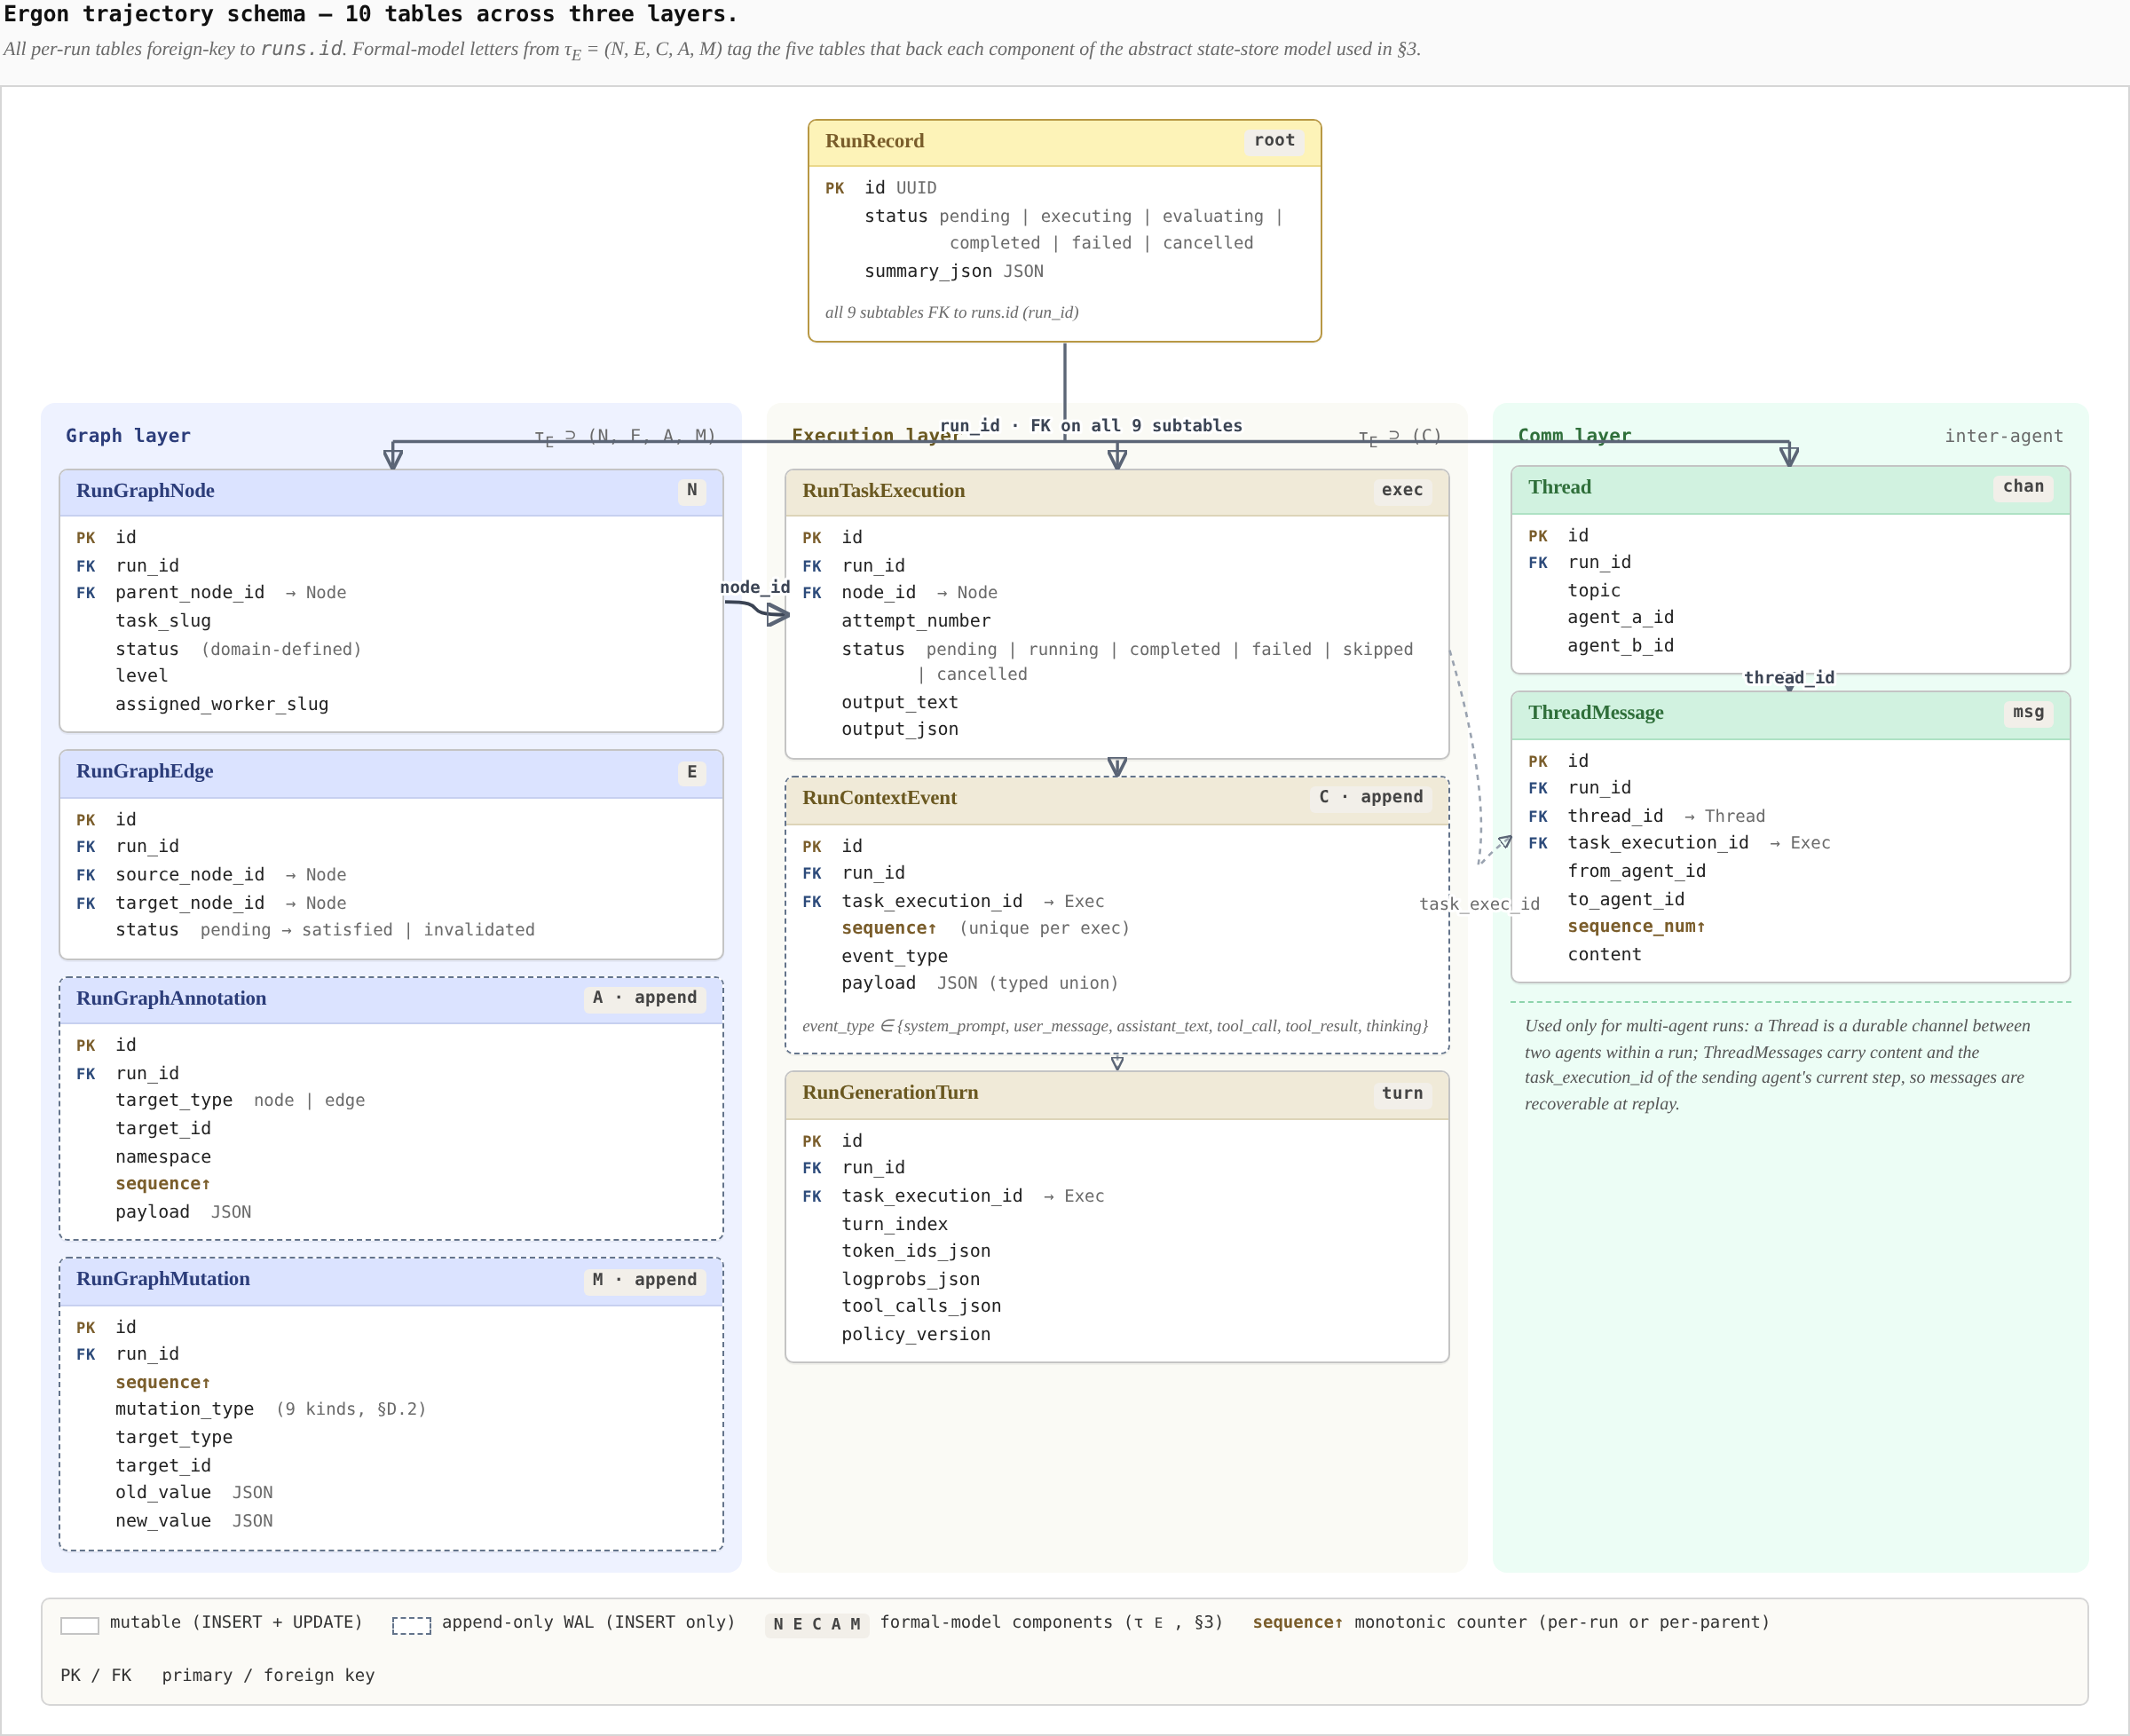
\includegraphics[width=1.15\linewidth]{ergon_schema.png}}
\caption{Ergon's ten-table trajectory schema. All per-run
tables foreign-key to \texttt{runs.id}; the formal-model tags
\texttt{[N]}, \texttt{[E]}, \texttt{[C]}, \texttt{[A]},
\texttt{[M]} identify the five tables that back each component
of $\tau_E$. Dashed borders mark append-only write-ahead-log
tables (INSERT only); solid borders mark mutable tables (INSERT
+ UPDATE). The single cross-group foreign key
\texttt{node\_id}: Execution~$\to$~Node is the join that lets
reasoning events and generation turns recover their position
in the task DAG.}
\label{fig:schema}
\end{figure}

\paragraph{Graph layer.} \texttt{RunGraphNode}
(\texttt{persistence/graph/models.py:L44-L89}) stores the
containment tree directly --- each node carries its own
\texttt{parent\_node\_id} and integer \texttt{level}, so the
full hierarchy is one indexed SELECT rather than a recursive
CTE. \texttt{RunGraphEdge} (\texttt{:L96-L116}) stores data
dependencies with status $\in\{$\texttt{pending},
\texttt{satisfied}, \texttt{invalidated}$\}$.
\texttt{RunGraphAnnotation} (\texttt{:L123-L165}) and
\texttt{RunGraphMutation} (\texttt{:L172-L186}) are both
append-only: each carries a per-run monotonic
\texttt{sequence}, and any state at any past point in a run is
reconstructed by replaying mutations up to that sequence
against an empty graph. Annotations additionally carry a
\texttt{namespace} so multiple subsystems (experiment config,
trainer hints, dashboard state) can version their metadata
independently on the same target.

\paragraph{Execution layer.} \texttt{RunTaskExecution}
(\texttt{persistence/telemetry/models.py:L96-L157}) wraps one
attempt at a node: if a worker retries, each attempt gets its
own row with an incremented \texttt{attempt\_number}, so the
context events and generation turns of failed attempts are
preserved alongside the successful one.
\texttt{RunContextEvent} (\texttt{persistence/context/models.py:L25-L49})
is the typed reasoning log --- the substrate backing $C$. It
is append-only, with a \texttt{sequence} unique per
\texttt{task\_execution\_id}, and a discriminated-union
\texttt{payload} whose shape depends on \texttt{event\_type}:
\begin{description}[leftmargin=0pt,itemindent=0pt,labelindent=0pt,labelsep=0.4em,itemsep=1pt,topsep=2pt,parsep=0pt,font=\normalfont\bfseries]
\sloppy
\item[system\_prompt, user\_message:] plain \texttt{text}
  (user messages additionally carry \texttt{from\_worker\_key}
  to attribute inter-worker sends).
\item[assistant\_text, thinking:] \texttt{text},
  \texttt{turn\_id}, and optional \texttt{turn\_token\_ids} /
  \texttt{turn\_logprobs} (populated for vLLM, absent for
  cloud APIs that do not expose token-level information).
\item[tool\_call:] \texttt{tool\_call\_id}, \texttt{tool\_name},
  \texttt{args}, plus the same token/logprob fields.
\item[tool\_result:] \texttt{tool\_call\_id},
  \texttt{tool\_name}, \texttt{result}, \texttt{is\_error}.
\end{description}
\texttt{RunGenerationTurn}
(\texttt{persistence/telemetry/models.py:L383-L464}) is the
per-model-call convenience extraction: one row per call, with
the raw response object, an extracted \texttt{response\_text},
\texttt{token\_ids\_json}, \texttt{logprobs\_json}, and
\texttt{tool\_calls\_json}. It is redundant with
\texttt{RunContextEvent} --- the event log is the substrate,
the turn table is a reader-friendly index --- but carrying
both avoids rehydrating token arrays from event payloads on
every training step.

\paragraph{Communication layer.} \texttt{Thread}
(\texttt{persistence/telemetry/models.py:L343-L353}) and
\texttt{ThreadMessage} (\texttt{:L360-L376}) are used only by
multi-agent runs. A thread is a durable channel between two
named agents within a run; each \texttt{ThreadMessage} carries
the sending agent's current \texttt{task\_execution\_id}, so a
replay can recover which reasoning step authored which
message. Single-agent runs leave both tables empty.

\paragraph{Engine.} The production deployment is PostgreSQL
15; SQLite is used only for test fixtures, which forces JSON
payload columns to use the broadly portable \texttt{JSON} type
rather than \texttt{JSONB}. The consequence is that projection
code (\S\ref{app:projections}) must read JSON payloads
client-side rather than push them through Postgres path
operators, but this is cheap because projections run at export
time, not on the rollout hot path. Migrations are managed by
Alembic at \texttt{ergon\_core/migrations/}.

\subsection{Mutation Kinds}
\label{app:system:mutations}

Every change to the run graph flows through a single
dispatcher, \texttt{GraphRepository.\_log\_mutation}
(\texttt{ergon\_core/core/runtime/services/}\allowbreak\texttt{graph\_repository.py:L848-L890}),
which allocates the next per-run \texttt{sequence} (line
L848-L856: \texttt{SELECT MAX(sequence)+1} within the current
run), writes one \texttt{RunGraphMutation} row with
\texttt{old\_value}/\texttt{new\_value} snapshots, and fires
registered listeners asynchronously. Mutations are strictly
append-only: reversals produce new mutations, not edits to
prior ones; deletions are tombstones (see
\texttt{annotation.deleted} below). The system defines nine
mutation kinds (literal declaration at
\texttt{persistence/graph/models.py:L24-L34}), summarised in
Table~\ref{tab:mutations}.

\begin{table}[h]
\centering
\small
\caption{The nine mutation kinds. \emph{Payload} lists the
domain-specific fields beyond the common
\texttt{(sequence, target\_type, target\_id, actor,
old\_value, new\_value)}. \emph{Invariants} are checked in the
dispatch path at
\texttt{runtime/services/graph\_repository.py}; when no entry
appears, the repository performs no domain validation and
defers enforcement to the experiment layer (per the repository
contract at \texttt{graph\_repository.py:L7-L9}).}
\label{tab:mutations}
\footnotesize
\setlength{\tabcolsep}{3pt}
\begin{tabular}{@{}l>{\raggedright\arraybackslash}p{0.22\linewidth}>{\raggedright\arraybackslash}p{0.42\linewidth}l@{}}
\toprule
\textbf{Kind} & \textbf{Payload} & \textbf{Invariants} & \textbf{File:L-L} \\
\midrule
\texttt{node.added}            & \texttt{task\_slug}, \texttt{instance\_key}, \texttt{description}, \texttt{status}, \texttt{assigned\_worker\_slug} & None.                                                                                                                               & \texttt{:L302-L312} \\
\texttt{node.removed}          & (same as above)                                                                                             & Cascades \texttt{edge.removed} for all incident edges first, then marks node terminal (node rows are not deleted).                  & \texttt{:L314-L358} \\
\texttt{node.status\_changed}  & \texttt{status}                                                                                             & If \texttt{only\_if\_not\_terminal=True}, skip if already in \{\texttt{COMPLETED}, \texttt{FAILED}, \texttt{CANCELLED}\}.            & \texttt{:L360-L400} \\
\texttt{node.field\_changed}   & \texttt{field}, \texttt{value}                                                                              & \texttt{field}~$\in$~\{\texttt{description}, \texttt{assigned\_worker\_slug}\} (whitelist at \texttt{:L62}); else \texttt{ValueError}. & \texttt{:L402-L434} \\
\texttt{edge.added}            & \texttt{source\_node\_id}, \texttt{target\_node\_id}, \texttt{status}                                       & Both endpoints must exist (\texttt{DanglingEdgeError}); new edge must not create a cycle (DFS at \texttt{:L892-L915}).              & \texttt{:L438-L474} \\
\texttt{edge.removed}          & (same as above)                                                                                             & None; edge row marked terminal (not deleted).                                                                                       & \texttt{:L476-L502} \\
\texttt{edge.status\_changed}  & \texttt{status}                                                                                             & None at repo layer; lifecycle \texttt{pending}~$\to$~\texttt{satisfied} / \texttt{invalidated} is experiment-layer policy.          & \texttt{:L504-L531} \\
\texttt{annotation.set}        & \texttt{namespace}, \texttt{payload}                                                                        & None; each call inserts a new annotation row (no upsert). Latest \texttt{sequence} within namespace is the current value.           & \texttt{:L535-L573} \\
\texttt{annotation.deleted}    & \texttt{namespace}, \texttt{payload}                                                                        & Soft delete: inserts a tombstone row with empty payload so the append-only log retains full history.                                & \texttt{:L647-L685} \\
\bottomrule
\end{tabular}
\end{table}

Three invariants are worth calling out because they resolve
otherwise-tricky concurrent-write conditions without
distributed coordination:

\paragraph{Acyclicity on \texttt{edge.added}
(\texttt{:L892-L915}).} Each \texttt{edge.added} runs a DFS
from \texttt{target\_node\_id} following outgoing edges; if
the walk reaches \texttt{source\_node\_id}, the insertion is
rejected with \texttt{CycleError}. Enforcing this at the
repository rather than the experiment layer means every run
graph is a DAG by construction, which is what downstream
projections ($\pi_{\text{call-tree}}$,
$\pi_{\text{per-agent}}$) rely on for their topological walks.

\paragraph{Terminal-write guard on
\texttt{node.status\_changed} (\texttt{:L381-L382}).} When
called with \texttt{only\_if\_not\_terminal=True}, the mutation
is skipped if the node already holds a terminal status
(\texttt{COMPLETED}, \texttt{FAILED}, or \texttt{CANCELLED}
per \texttt{status\_conventions.py:L23}). This single check
resolves cascade-cancellation races: concurrent paths that
both attempt to write a terminal status converge on
first-writer-wins without requiring a distributed lock.

\paragraph{Tombstone semantics on
\texttt{annotation.deleted} (\texttt{:L662-L672}).} A
``deletion'' inserts a new annotation row with an empty
payload rather than removing prior rows. This preserves the
ability to replay the full annotation timeline --- the
diagnostic dashboards and the counterfactual-replay tooling
both depend on being able to reconstruct every historical
payload at any sequence, including the ones that were later
cleared.

\paragraph{Edge-status lifecycle.} Conventionally
\texttt{pending}~$\to$~\texttt{satisfied} on dependency
resolution and \texttt{pending}~$\to$~\texttt{invalidated} on
upstream cancellation; backward transitions are not
prevented at the repository, but the experiment layer that
schedules workers treats \texttt{invalidated} as terminal.
The string values are constants in
\texttt{status\_conventions.py:L30-L32} and are not enforced
by a DB-level check constraint --- custom experiment graphs
are free to add their own edge statuses, at the cost of being
invisible to default dashboards.

\subsection{Trainer Adapters}
\label{app:verl}

Ergon decouples rollout execution from trainer execution by
serving a small HTTP surface that all three supported trainers
(TRL, VERL, OpenRLHF) consume. The server is a FastAPI
application at \texttt{ergon\_core/core/api/rollouts.py:L24-L89};
trainer-side adapters are
$<100$-line shims in
\texttt{ergon\_infra/ergon\_infra/adapters/}. The trainers pull;
the server never pushes.

\paragraph{Endpoints.} Four routes, all under
\texttt{/rollouts}. \texttt{POST /submit} accepts a
\texttt{SubmitRequest} (\texttt{core/rl/rollout\_types.py:L21-L35})
carrying \texttt{definition\_id}, \texttt{num\_episodes},
\texttt{policy\_version}, and an optional
\texttt{model\_target\_override}; it returns
\texttt{SubmitResponse} with a \texttt{batch\_id}, a list of
\texttt{run\_ids}, and the initial \texttt{BatchStatus} (status
202). \texttt{GET /\{batch\_id\}} returns a \texttt{PollResponse}
(\texttt{:L61-L69}) with \texttt{status}, \texttt{completed},
\texttt{total}, the ordered list of completed
\texttt{Trajectory}~objects, and a list of
\texttt{EpisodeFailure}~records for any runs that crashed.
\texttt{DELETE /\{batch\_id\}} cancels an in-flight batch.
\texttt{POST /sync-weights} triggers an optional vLLM reload
for full-weight RFT scenarios (\texttt{:L67-L88}). Batch and
per-episode state are persisted in Postgres
(\texttt{RolloutBatch}, \texttt{RolloutBatchRun}), so trainers
can resume polling after either a trainer-side or server-side
restart.

\paragraph{Intermediate representation.} The
\texttt{Trajectory} object (\texttt{rollout\_types.py:L38-L51})
is the one wire-format contract the three adapters share. It
is a flat tuple:
\begin{center}
\texttt{(run\_id, agent\_id, prompt\_ids, completion\_ids,
logprobs, env\_mask, reward, num\_turns)}.
\end{center}
It is constructed at poll time by
\texttt{extract\_agent\_trajectories} in
\texttt{core/rl/extraction.py:L49-L117}. The extraction walks
the rollout's context events $C$ --- not its generation turns
--- so the wire format is grounded in the substrate's
append-only log rather than in a denormalised turn view.
Concretely: the function groups \texttt{RunContextEvent}~rows
by \texttt{worker\_binding\_key}, builds the prompt from the
initial \texttt{system\_prompt}/\texttt{user\_message} events,
and then walks the remaining events in sequence order.
Model-authored events (\texttt{assistant\_text},
\texttt{tool\_call}, \texttt{thinking}) contribute their
\texttt{turn\_token\_ids} to \texttt{completion\_ids} with
\texttt{env\_mask=1} and their \texttt{turn\_logprobs} to
\texttt{logprobs}; environment events (\texttt{tool\_result})
contribute tokenised text to \texttt{completion\_ids} with
\texttt{env\_mask=0} and zero-padded \texttt{logprobs}. The
scalar \texttt{reward} is attached by
\texttt{RewardStrategy.assign} (\texttt{extraction.py:L103})
from the run's \texttt{RunTaskEvaluation} rows. Because
$\tau_E$ is event-sourced, the entire IR is reproducible at
export time against the pinned Postgres row versions --- the
same rollout replayed tomorrow produces byte-identical IR.

\paragraph{Adapters.} Each adapter is a shim that calls
\texttt{submit}, polls \texttt{\{batch\_id\}}, and maps the
returned \texttt{Trajectory} into the native batch type the
trainer expects. Table~\ref{tab:adapters} summarises; the
longest file is $\sim$90 lines.

\begin{table}[h]
\centering
\small
\caption{Trainer adapters. All three are thin shims over the
shared \texttt{/rollouts} endpoints; the framework-specific
work is field renaming and wrapping in the native batch type.}
\label{tab:adapters}
\begin{tabular}{@{}l>{\raggedright\arraybackslash}p{0.24\linewidth}>{\raggedright\arraybackslash}p{0.20\linewidth}>{\raggedright\arraybackslash}p{0.34\linewidth}@{}}
\toprule
\textbf{Trainer} & \textbf{Adapter file} & \textbf{Output type} & \textbf{Field renames and quirks} \\
\midrule
TRL (GRPO) & \texttt{trl\_http.py:L25-L91} & \texttt{dict} (GRPOTrainer contract) & \texttt{reward}~$\to$~\texttt{completion\_reward}; synchronous \texttt{httpx.Client}; batch of $n$ trajectories per call. \\
VERL       & \texttt{verl\_http.py:L23-L82} & \texttt{AgentLoopOutput} & \texttt{completion\_ids} $\to$ \texttt{response\_ids}; \texttt{env\_mask} $\to$ \texttt{response\_mask}; async; single episode per call (streaming integration). \\
OpenRLHF   & \texttt{openrlhf\_http.py}\allowbreak\texttt{:L24-L84} & \texttt{dict} (\texttt{input\_ids}, \texttt{response\_ids}, \texttt{logprobs}, \texttt{reward}) & Drops \texttt{env\_mask} (OpenRLHF's return shape does not carry turn masks); module-level \texttt{configure()} for one-time setup; async; single episode per call. \\
\bottomrule
\end{tabular}
\end{table}

Because the trainers consume the same \texttt{Trajectory}
contract, a model trained under one trainer can be evaluated
against another trainer's harness without re-exporting: the
Ergon substrate is written once, and the format difference is
absorbed in the adapter layer. A new trainer is added by
writing one adapter file; no changes to the substrate, the
server, or the existing adapters are required. The repository
ships no SkyRL adapter at submission time, but the pattern
supports one at the same cost as the existing three.


% ----------------------------------------------------------------------------
% Appendix E --- Tech-Stack Integrations List.
% Reframed (v5.6) from v4's Extended Community / Framework Capability Matrix.
% Purpose: descriptive list of what Ergon plugs into / exports to --- at the
% agents layer (Pydantic AI, LangGraph, CrewAI, AutoGen, Google ADK, Claude
% Code), RL layer (TRL, VERL, OpenRLHF, SkyRL, ProRL Agent, AReaL, AgentGym-RL,
% RAGEN, MARTI, etc.), and trajectory-format export targets (the five
% projections' canonical formats). Not a normative capability matrix; a
% descriptive integrations map.
% Content: written fresh in Session 11, filling in real integration status.
% Framing: "Ergon hosts existing agent frameworks (X, Y, Z) via adapters,
% feeds existing RL trainers (A, B, C) via projections, and exports to the
% five community canonical trajectory formats surveyed in Sec.~2.2."
% ----------------------------------------------------------------------------

\section{Tech-Stack Integrations}
\label{app:integrations}

This appendix is a descriptive integrations \emph{map}, not a
normative capability matrix. For each of three layers --- agent
frameworks the substrate hosts as inner runtimes, RL trainers
the substrate feeds via HTTP adapters, and canonical trajectory
formats the substrate projects to --- we list the concrete
integrations shipped at submission time, together with the
integrations on the near-term roadmap. Rows marked
\emph{integrated} are exercised by the experiments in
\S\ref{sec:validation} or by the Ergon test suite; rows marked
\emph{planned} are scoped in RFCs in the Ergon repository under
\texttt{docs/rfcs/active/} and do not contribute to any result
reported in this paper.

\paragraph{Agents layer.} Ergon hosts third-party agent loops
as inner runtimes behind an \texttt{AgentRuntimeAdapter}
contract: the adapter wraps the framework's loop, serialises
each turn as a \texttt{RunContextEvent} (see
\S\ref{app:system:postgres}), and replays stored events to
reconstruct framework-native message state on resumption. One
adapter ships today; five are scoped
(Table~\ref{tab:integrations:agents}).

\begin{table}[h]
\centering
\small
\setlength{\tabcolsep}{4pt}
\caption{Agent-framework integrations. Integrated rows are
exercised by the flexible-agent worker. Planned rows are scoped
in the referenced RFC in the Ergon repository.}
\label{tab:integrations:agents}
\begin{tabular}{@{}l l >{\raggedright\arraybackslash}p{0.42\linewidth}@{}}
\toprule
\textbf{Framework} & \textbf{Status} & \textbf{Evidence / RFC} \\
\midrule
Pydantic AI  & integrated & \texttt{workers/baselines/}\allowbreak\texttt{react\_worker.py:L28-L105} wraps \texttt{Agent.iter()}; context replay at \texttt{persistence/context/}\allowbreak\texttt{assembly.py:L94-L130} \\
LangGraph    & planned    & \texttt{agent-framework-adapter-layer} (state-graph replay) \\
CrewAI       & planned    & \texttt{agent-framework-adapter-layer} (task-delegation shim) \\
AutoGen      & planned    & \texttt{agent-framework-adapter-layer} (per-agent \texttt{worker\_binding\_key}) \\
Google ADK   & planned    & \texttt{agent-framework-adapter-layer} (state-machine replay) \\
Claude Code  & planned    & \texttt{agent-framework-adapter-layer} (closest native fit) \\
\bottomrule
\end{tabular}
\end{table}

\paragraph{RL trainers.} Ergon serves a FastAPI
\texttt{/rollouts} surface consumed by framework-specific
shims; the handshake is documented in Appendix~\ref{app:verl}.
Three shims ship today --- TRL, VERL, OpenRLHF --- each
$\sim$80--90 lines. Six are scoped
(Table~\ref{tab:integrations:trainers}).

\begin{table}[h]
\centering
\small
\setlength{\tabcolsep}{4pt}
\caption{RL-trainer integrations. Integrated rows are the three
adapters compared in Table~\ref{tab:adapters}. Planned rows are
scoped in \texttt{rl-trainer-adapter-expansion}, which also
formalises the HTTP handshake as a \texttt{TrainerHttpAdapter}
\mbox{Protocol}.}
\label{tab:integrations:trainers}
\begin{tabular}{@{}l l >{\raggedright\arraybackslash}p{0.42\linewidth}@{}}
\toprule
\textbf{Trainer} & \textbf{Status} & \textbf{Evidence / RFC} \\
\midrule
TRL (GRPO)   & integrated & \texttt{adapters/trl\_http.py:L1-L92} \\
VERL         & integrated & \texttt{adapters/verl\_http.py:L1-L83} (\texttt{@register("ergon")}) \\
OpenRLHF     & integrated & \texttt{adapters/openrlhf\_http.py:L1-L85} \\
SkyRL        & planned    & \texttt{rl-trainer-adapter-expansion} \\
ProRL Agent  & planned    & \texttt{rl-trainer-adapter-expansion} \\
AReaL        & planned    & \texttt{rl-trainer-adapter-expansion} \\
AgentGym-RL  & planned    & \texttt{rl-trainer-adapter-expansion} \\
RAGEN        & planned    & \texttt{rl-trainer-adapter-expansion} \\
MARTI        & planned    & \texttt{rl-trainer-adapter-expansion} \\
\bottomrule
\end{tabular}
\end{table}

\paragraph{Projection / export formats.} The five canonical
trajectory shapes surveyed in \S\ref{sec:system:format} each
correspond to a projection operator over the substrate. Two
ship today (step-indexed tuples and per-agent streams, both
produced by \texttt{extract\_agent\_trajectories} at
\texttt{core/rl/extraction.py:L49-L117}); three are scoped
(Table~\ref{tab:integrations:projections}). The three planned
projections are pure reads over the existing schema
(option-tagged, call-tree) or reserve a new annotation
namespace (MCTS) --- no DB migration is required for any of
them.

\begin{table}[h]
\centering
\small
\setlength{\tabcolsep}{4pt}
\caption{Projection-operator integrations. The five shapes map
to the trajectory-format survey in \S\ref{sec:system:format}.
Planned rows are one RFC each.}
\label{tab:integrations:projections}
\begin{tabular}{@{}l l >{\raggedright\arraybackslash}p{0.42\linewidth}@{}}
\toprule
\textbf{Projection} & \textbf{Status} & \textbf{Evidence / RFC} \\
\midrule
Step-indexed tuples    & integrated & \texttt{core/rl/extraction.py:L49-L117} \\
Per-agent streams      & integrated & same, keyed by \texttt{worker\_binding\_key} \\
Option-tagged (semi-MDP) & planned  & \texttt{projection-operator-option-tagged} \\
Call-tree (nested)     & planned    & \texttt{projection-operator-call-tree} \\
MCTS search-tree       & planned    & \texttt{projection-operator-mcts} (\texttt{mcts.*} annotation namespace) \\
\bottomrule
\end{tabular}
\end{table}

Of the twenty rows in the three tables, six are integrated and
fourteen are planned. The integrated subset is sufficient for
the experiments reported in \S\ref{sec:validation}; the planned
subset is what Ergon must ship to fully back the substrate
framing of \S\ref{sec:system}. Each planned RFC scopes the
code additions required and notes the paper-parity dependency
explicitly.

% ----------------------------------------------------------------------------
% Appendix F --- Experimental Setup. Consolidates former appendices F (Agent
% Action Spaces), G (Benchmark Details), H (Flexible Agent and Projection
% Details), and I (Cross-harness Reconciliation Methodology) into one
% themed appendix. Old \section labels are preserved as \label aliases on
% the new subsections so body refs (\ref{app:reconciliation},
% \ref{app:benchmarks}) continue to resolve.
% ----------------------------------------------------------------------------

\section{Experimental Setup}
\label{app:setup}

This appendix consolidates the experimental-setup details supporting
\S\ref{sec:validation}: per-benchmark agent action spaces
(\S\ref{app:actions}), benchmark selection and statistics
(\S\ref{app:benchmarks}), the flexible-agent scaffold used as the
workload-generating system (\S\ref{app:fivescaffolds}), and the
cross-harness reconciliation methodology for the SWE-Bench Verified
comparison (\S\ref{app:reconciliation}).

\subsection{Agent action spaces}
\label{app:actions}

Table~\ref{tab:actions} lists the full action space available to
the flexible-agent worker on each benchmark. Every benchmark
agent has access to the four subtask-decomposition tools (shared
across all benchmarks); task-specific tools vary.

\begin{table}[h]
\centering
\small
\caption{Per-benchmark agent action space. The four
subtask-decomposition tools are shared across all benchmarks;
remaining tools are task-specific.}
\label{tab:actions}
\begin{tabular}{@{}lll@{}}
\toprule
\textbf{Benchmark} & \textbf{Tool} & \textbf{What it does} \\
\midrule
\textit{All} & \texttt{spawn\_subtask} & Create a child subtask with a description and required inputs \\
\textit{All} & \texttt{cancel\_subtask} & Cancel a subtask by ID (late cancellation is distinct from completion) \\
\textit{All} & \texttt{wait\_on\_subtask} & Block on a subtask ID until it reaches a terminal status \\
\textit{All} & \texttt{report\_result} & Write this task's result and mark the task complete \\
\midrule
MiniF2F & \texttt{lean\_repl} & \todo{short description} \\
MiniF2F & \texttt{lean\_check} & \todo{short description} \\
\midrule
Research Rubrics & \texttt{web\_search} & \todo{short description (Tavily)} \\
Research Rubrics & \texttt{read\_document} & \todo{short description (httpx+trafilatura)} \\
\midrule
SWE-Bench Verified & \texttt{bash} & \todo{short description} \\
SWE-Bench Verified & \texttt{edit\_file} & \todo{short description} \\
\bottomrule
\end{tabular}
\end{table}

The subtask-decomposition tools are exposed uniformly: the
worker's system prompt describes them mechanically and gives no
guidance on when to use them, so observed delegation structure
comes from the agent rather than from prompting (see
\S\ref{sec:validation:setup}).


\subsection{Benchmark details}
\label{app:benchmarks}

\placeholder{0.95}{%
  \textbf{Table A2: MiniF2F problem selection.}
  Difficulty levels, problem categories, proof-length statistics,
  subset used in \S\ref{sec:validation}.
}

\placeholder{0.95}{%
  \textbf{Table A3: Research Rubrics question distribution.}
  Topic distribution, rubric criteria counts, evaluator
  configuration.
}

\placeholder{0.95}{%
  \textbf{Table A4: SWE-Bench Verified subset.}
  Per-repository counts in the 100--150 instance subset used in
  \S\ref{sec:validation}, sampling procedure, comparison to full
  Verified statistics, E2B template details.
}


\subsection{Flexible agent and projection details}
\label{app:fivescaffolds}

\subsubsection{Benchmark delegation toolkit}
\label{app:benchmark-action-space}

The flexible-agent worker of \S\ref{sec:validation} is given a
particular set of delegation actions that mutate the substrate.
This action space is a design choice of our benchmark, not a
feature of Ergon itself --- another research team could expose a
different set of delegation actions against the same substrate
and run a different benchmark. The toolkit we expose consists of
six verbs, each corresponding to a named mutation pattern on
$(N, E, A)$:
\begin{itemize}\itemsep 0pt
  \item \texttt{add\_subtask}: creates a single child node and
    dispatches it for asynchronous execution.
  \item \texttt{plan\_subtasks}: atomically creates a sub-DAG of
    children validated by Kahn's algorithm, with root children
    dispatched to a concurrency-15 executor.
  \item \texttt{cancel\_task}: marks a node terminal, cascades to
    descendants, and invalidates outgoing dependency edges
    (cancelled sub-trees remain in $(N, E)$ for analysis).
  \item \texttt{refine\_task}: edits a non-running node's
    description with field-history preserved.
  \item \texttt{restart\_task}: resets a terminal node to
    \textsc{pending} and cascades invalidation to downstream
    dependencies.
  \item \texttt{list\_subtasks} and \texttt{get\_subtask}:
    read-only observations of the current containment tree.
\end{itemize}
Each verb maps to a named mutation type in $M$, so downstream
evaluators distinguish delegation, cancellation, and refinement
from ordinary tool use without custom parsing --- independently
of what specific verbs our benchmark chose to expose.

\subsubsection{Agent details and projections}

\todo{For the flexible-agent worker of \S\ref{sec:validation}:
system prompt, full tool inventory (benchmark action space above
plus task-specific tools), one-shot example if any, and the
turn-budget and stopping rules. For each of the five projection
operators $\pi_{\text{step}}$, $\pi_{\text{per-agent}}$,
$\pi_{\text{call-tree}}$, $\pi_{\text{macro}}$,
$\pi_{\text{json-log}}$: one worked example on one trajectory
from each task family, the drops manifest it produces, and
discussion of which behavioural metrics each projection
structurally cannot preserve.}


% ----------------------------------------------------------------------------
% Appendix I (Dataset Onboarding Guide), Appendix J (Automated Experimental
% Infrastructure), and Appendix K (Fault-Injection Methodology) were cut in
% 2026-04-21. Rationale: all three had zero body-text citations (or the one
% K cite was rewritten to point at Appendix D's WAL/mutation-log invariants).
% I was a how-to-use-Ergon tutorial that belongs in the repo README; J was
% orchestration lore that belongs in the repo README; K (fault injection) is
% not part of the new experiment setup. Downstream appendices (formerly L/M/N)
% are automatically relabelled to I/J/K by LaTeX's \section counter; no
% manual renumbering needed.
% ----------------------------------------------------------------------------


\subsection{Cross-harness reconciliation methodology}
\label{app:reconciliation}

\todo{Session 11: Cross-harness reconciliation methodology appendix. Source: Weekend 1 Sec.~4.5 experiment.
Structure: (a) convention specification --- union convention justified against alternatives (SWE-agent's convention, Agentless's convention, minimal common denominator); (b) download and re-grading code walkthrough; (c) what the re-grading preserves vs what it cannot preserve (explicit drops manifest for the reconciliation convention itself); (d) drops manifests for the SWE-agent $\to$ rollout-card and Agentless $\to$ rollout-card ingestions per Sec.~4.2 ``Cross-harness reconciliation''; (e) \texttt{no\_generation} convention analysis --- 50 instances SWE-agent, 4 Agentless; why Convention A (exclude) and Convention B (include as zero) bracket the reasonable range of harness-level choices.}

% ----------------------------------------------------------------------------
% Appendix J (Additional Rollout Traces) was cut in 2026-04-21. The per-
% benchmark trace figures (Fig A3 MiniF2F, Fig A4 Research Rubrics, Fig A5
% SWE-Bench Verified) were dropped --- they add rollout colour but don't
% back any claim. The crown-jewel six-projection figure (formerly Fig A2)
% was relocated to Appendix C (app:projections) as Fig~\ref{fig:sixproj}
% since it is the visual statement of the projection-loss argument that
% appendix makes in prose. LaTeX auto-renumbers the Benchmark Card below
% from appendix K to J.
% ----------------------------------------------------------------------------

% ----------------------------------------------------------------------------
% Appendix G --- Behavioural Quantities (moved from §4.2 body on 2026-04-22
% per signposting / length pass; see proposed_edits_signposting.md C6).
% ----------------------------------------------------------------------------

\section{Behavioural Quantities}
\label{app:quantities}

This appendix catalogues the six behavioural quantities
referenced in \S\ref{sec:validation:setup}. Each is a
canonical analysis of one of the five research communities
surveyed in \S\ref{sec:problem:communities}. The set is
illustrative: a rollout card supports arbitrarily many
analyses, and the three quantities exercised in
\S\ref{sec:validation:results} (abandonment ratio by depth,
per-agent sibling embedding distance, and the
\texttt{no\_generation} split in the SWE-bench reconciliation)
are drawn from this set.

\begin{table}[h]
\centering
\small
\caption{Six behavioural quantities exercised in
\S\ref{sec:validation:results}, each the canonical analysis of
one of the five research communities from
\S\ref{sec:problem:communities}. The set is illustrative: a
rollout card supports arbitrarily many such analyses.}
\label{tab:quantities}
\begin{tabular}{@{}p{0.32\textwidth}p{0.28\textwidth}p{0.32\textwidth}@{}}
\toprule
\textbf{Quantity} & \textbf{Community} & \textbf{Computed from} \\
\midrule
Step-indexed return under episode mask & Long-horizon LLM-agentic RL \citep{chen2025loop, wang2025ragen} & \texttt{events.jsonl} token spans \\
Option termination frequency & HRL / macro-action \citep{bacon2017optioncritic} & \texttt{mutations.jsonl} status transitions \\
Call-tree depth distribution & Recursive LMs \citep{zhu2024redel} & \texttt{nodes.jsonl} \texttt{parent\_id} chains \\
Per-agent sibling embedding distance & Fixed-role MAS \citep{cemri2025mast} & \texttt{nodes.jsonl} + \texttt{events.jsonl} \\
Node visit entropy across frontier & MCTS-based training \citep{rstarmath2025, feng2024restmcts} & \texttt{annotations.jsonl} (MCTS namespace) \\
Dispatch-and-wait rate & Async MAS & \texttt{events.jsonl} + \texttt{mutations.jsonl} \\
\bottomrule
\end{tabular}
\end{table}

% ----------------------------------------------------------------------------
% Appendix J --- Benchmark Card: Evaluative Role, Assumptions, Limitations.
% CARRY VERBATIM.
% ----------------------------------------------------------------------------

\section{Benchmark Card: Evaluative Role, Assumptions, and Limitations}
\label{app:benchmarkcard}

\paragraph{Evaluative role.}
The Ergon benchmark suite, paired with the trajectory
representation and projection operators, supports evaluative
claims about dynamic-delegation agents that were previously not
comparable across research communities: (i) whether an agent
uses concurrent dispatch when it is available; (ii) whether an
agent cancels sub-tasks that are not making progress; (iii)
whether an agent's delegation structure contains dependency
diamonds that exceed tree-shape formalisms; (iv) whether the
agent's reasoning expresses intent that its recorded structural
actions fail to realise; (v) whether a community's preferred
trajectory format preserves each of these behaviours under its
projection operator.

\paragraph{Assumptions.}
\begin{itemize}
  \item The tool implementations (web search, document retrieval,
    Lean REPL, SWE-Bench harness) are stable at their released
    versions and latency distributions; substantial drift in
    tool-provider behaviour may invalidate fault-injection
    calibration.
  \item The rubric-based evaluator (GPT-4o-mini, for Research
    Rubrics) is treated as a noisy but calibrated judge; we do not
    claim evaluator infallibility and provide inter-rater agreement
    statistics in Appendix~\ref{app:benchmarks}.
  \item The flexible-agent worker is given access to the
    subtask-decomposition tools but not prompted to use them;
    observed delegation structure reflects the backbone model's
    untutored decomposition under a minimal system prompt, not a
    researcher-imposed strategy.
\end{itemize}

\paragraph{Limitations.}
\begin{itemize}
  \item Three task families; generalisation claims to other
    long-horizon settings should be made cautiously. The
    behavioural coverage of \S\ref{sec:validation} is complementary
    but not exhaustive.
  \item LLM-judge failure modes (reward hacking, distribution
    shift) are documented but not fully characterised.
  \item Tool-provider API drift may require re-calibration;
    reproducibility bundle pins tool-provider snapshots. SWE-Bench
    Verified's per-repository environment specs are pinned to the
    \texttt{swebench} package version used.
\end{itemize}

\paragraph{Intended use.}
Evaluation of dynamic-delegation policies via the substrate and
projection-preservation framework. The benchmark suite is \emph{not}
intended as a stand-alone prover, a factual QA benchmark, or a
general agentic capability test; claims in those directions should
use purpose-built benchmarks and metrics.

\paragraph{Failure modes.}
Rubric reward hacking on Research Rubrics; MiniF2F proof leakage
from the backbone's training data; SWE-Bench test-pattern overfit
on popular repositories; tool-provider API drift; LLM-judge
sycophancy.



% ============================================================================
% Mandatory NeurIPS 2026 Paper Checklist
% ============================================================================
\input{checklist.tex}

\end{document}
